\documentclass[10pt,a4paper]{article}
\usepackage[utf8]{inputenc}
\usepackage[T1]{fontenc}
\usepackage[spanish,es-noquoting,es-nodecimaldot]{babel}
\usepackage[margin=1.8cm]{geometry}
\usepackage{amsmath,amssymb,amsfonts,bm}
\usepackage{graphicx}
\usepackage{booktabs}
\usepackage{adjustbox}
\usepackage{float}
\usepackage{caption}
\usepackage{xcolor}
\usepackage{hyperref}
\usepackage{microtype}
\DisableLigatures[-]{encoding = T1, family = tt*}
\usepackage{listings}
\usepackage{tikz}
\usetikzlibrary{shapes,arrows.meta,positioning,fit,backgrounds}

\definecolor{darkblue}{rgb}{0.0,0.16,0.52}
\definecolor{codegray}{rgb}{0.96,0.96,0.96}
\definecolor{codeborder}{rgb}{0.78,0.78,0.78}
\definecolor{s1col}{rgb}{0.86,0.96,0.90}
\definecolor{s2col}{rgb}{0.88,0.93,1.00}
\definecolor{s3col}{rgb}{1.00,0.95,0.84}
\definecolor{s4col}{rgb}{0.98,0.89,0.93}
\definecolor{s5col}{rgb}{0.92,0.89,0.98}
\definecolor{warnbg}{rgb}{1.00,0.96,0.90}
\definecolor{warnbd}{rgb}{0.82,0.42,0.05}
\definecolor{okbg}{rgb}{0.92,0.98,0.94}
\definecolor{okbd}{rgb}{0.10,0.55,0.32}

\hypersetup{
    colorlinks=true,
    linkcolor=darkblue,
    citecolor=darkblue,
    urlcolor=darkblue,
    pdfauthor={RL-VMC Framework},
    pdftitle={Hoja de Ruta RL-MCMC y Benchmark Paso 1: Superando a RWMH en VMC Cuantico 1D}
}

\lstset{
    backgroundcolor=\color{codegray},
    basicstyle=\ttfamily\footnotesize,
    breaklines=true,
    showstringspaces=false,
    frame=single,
    rulecolor=\color{codeborder},
    xleftmargin=0.25cm,
    framexleftmargin=0.2cm,
    literate={á}{{\'a}}1 {é}{{\'e}}1 {í}{{\'i}}1 {ó}{{\'o}}1 {ú}{{\'u}}1 {ñ}{{\~n}}1 {Ñ}{{\~N}}1 {¿}{{?`}}1 {¡}{{!`}}1 {–}{{--}}1 {—}{{---}}1
}

\newcommand{\callout}[4]{%
\begin{center}
\fcolorbox{#1}{#2}{%
\begin{minipage}{0.95\textwidth}
\vspace{0.12cm}
\textbf{#3}\\[0.1cm]
#4
\vspace{0.12cm}
\end{minipage}}
\end{center}
}

\title{\textbf{\Large Superando a Random-Walk Metropolis-Hastings en VMC Cuántico 1D:\\
Diagnóstico Teórico del Colapso de TD3-CDLB, Hoja de Ruta Progresiva de 5 Pasos\\
e Implementación del Benchmark Paso 1 (Gradiente Exacto Reparametrizado,\\
Desacoplamiento de Deriva y Recompensas de Eficiencia)}\\[0.3cm]
\large Marco Matemático, Validación Piloto en 3 Sistemas CASSCF y Protocolo de Ejecución en Ayler}
\author{\textbf{RL-VMC Framework / Deep Deterministic Quantum Monte Carlo}}
\date{Noviembre 2026}

\begin{document}
\emergencystretch=2em
\maketitle

\begin{abstract}
En la campaña de ablación anterior ejecutada en Ayler (Benchmarks B1 y B2, Sección 14 de \texttt{NODAL\_CROSSING\_BENCHMARKS\_REPORT.pdf}), un control estricto a ancho de propuesta emparejado ($\sigma_{\mathrm{RWMH}} = \sigma_{\mathrm{RL}}$) reveló un diagnóstico contundente: en su formulación previa (\texttt{TD3Learner1D} por electrón + recompensa \texttt{cdlb} + modo \texttt{residual\_mala}), el actor neuronal \texttt{DeepSet} ignoraba la fuerza cuántica $\bm{F}_Q = \nabla\ln|\Psi|$, se aplanaba contra el techo $\sigma_{\max}$ y degeneraba esencialmente en un \textit{Random-Walk Metropolis-Hastings} (RWMH) isotrópico, quedando incluso $18\%\text{--}43\%$ por debajo de RWMH puro en $N=4, g=2.0$ y apenas empatando en $N=6, g=1.0$. Este reporte descompone con rigor matemático las \textbf{cuatro causas estructurales} detrás de dicho colapso: (i) la dilución $1/N$ en la asignación de crédito del crítico local $Q(s_i, a_i)$ de TD3, (ii) el sesgo entrópico de CDLB ($-\alpha\log q \propto \alpha N \ln\sigma$) que sacrifica la aceptación hasta $\alpha \approx 6\%\text{--}10\%$ degradando $\tau_{\mathrm{int}}(E)$ y $D_{\mathrm{KL}}^{\mathrm{spin}}$, (iii) el desbalance de escalas en las características de entrada más la deriva confinante impuesta $\tau\bm{F}_Q$, y (iv) la \textbf{maldición exponencial} $\alpha_{\mathrm{all}} \sim (\sigma_{\mathrm{well}}/\sigma)^N$ y la \textbf{Barrera de Pareto Unimodal} intrínseca a toda propuesta Gaussiana diagonal.

A partir de este diagnóstico, se formula una \textbf{Hoja de Ruta Progresiva de 5 Pasos} ordenada estrictamente de menor a mayor complejidad de implementación, y se implementa, valida y documenta el \textbf{Paso 1} (\texttt{run\_step1\_gradient\_reward\_benchmark.sh}): el benchmark más trivial de desplegar porque requiere \textbf{cero líneas de código nuevo} en \texttt{rl\_vmc}, reutilizando íntegramente clases ya presentes en la paquetería (\texttt{REINFORCELearner1D}, \texttt{TD3Learner1D}, \texttt{DeepSetNeuralProposal1D} en modo \texttt{full\_gaussian}, \texttt{MHSampler1D.step\_single\_electron} y las recompensas \texttt{log\_esjd}/\texttt{kappa\_jump}/\texttt{barker\_jump}). Seleccionamos tres sistemas CASSCF convergidos ($N_{\mathrm{basis}}=256, n_{\mathrm{core}}=0$) que trazan el colapso exponencial de RWMH: $N=4, g=2.0$ (puente directo con B1/B2), $N=6, g=5.0$ (quiebre de RWMH \texttt{all\_electrons} a $\mathrm{Acc}=3.1\%$) y $N=8, g=5.0$ (muro exponencial de 70 determinantes donde RWMH cae a $\mathrm{Acc}=0.6\%$). La validación piloto local ya arroja un resultado decisivo: al reemplazar TD3 por el gradiente exacto reparametrizado de \texttt{REINFORCELearner1D} con \texttt{full\_gaussian} y \texttt{log\_esjd}, \textbf{la misma red DeepSet recupera $71\times$ la sensibilidad a $\bm{F}_Q$}, aprende un sobre-relajamiento heterogéneo pozo-por-pozo con \textbf{aceptación constante $\approx 78\%\text{--}80\%$ para $N=4, 6, 8$}, alcanza \textbf{$\mathrm{ESJD} = 10.4\text{--}12.6\ \mathrm{Bohr}^2/\mathrm{paso}$ ($5\times\text{--}52.5\times$ superior a RWMH)} y reduce $\tau_{\mathrm{int}}(E)$ a \textbf{$1.2\text{--}1.6$ pasos} (muestreo casi i.i.d.\ insesgado). Simultáneamente, exhibe con claridad quirúrgica la Barrera de Pareto Unimodal ($\sim 0$ flips inter-pozo), demostrando por qué el Paso 4 (Mezcla Local + \textit{Pair-Swap} de 2 cuerpos con Balance Detallado exacto) culminará la superioridad global de RL-MCMC sobre cualquier sampler clásico.
\end{abstract}

\tableofcontents
\vspace{0.5cm}
\hrule
\vspace{0.5cm}

% ==============================================================================
\section{Marco Teórico y Diagnóstico Profundo: ¿Por Qué RL-MALA Legado Degeneró en RWMH?}
% ==============================================================================

\subsection{Hamiltoniano Físico, Función de Onda CASSCF y Balance Detallado Exacto}

Consideramos el sistema de $N = N_\uparrow + N_\downarrow$ electrones interactuantes confinados en un pozo armónico unidimensional con repulsión Coulombiana suavizada (\textit{soft-Coulomb}):
\begin{equation}
\hat{H} = \sum_{i=1}^{N} \left( -\frac{1}{2}\frac{\partial^2}{\partial x_i^2} + \frac{1}{2}\omega^2 x_i^2 \right) + \sum_{1 \le i < j \le N} \frac{g}{\sqrt{(x_i - x_j)^2 + a^2}}, \qquad \omega = 0.1,\; a = 0.1.
\label{eq:hamiltonian}
\end{equation}
Para aislar estrictamente el problema de \textbf{muestreo cuántico} del problema de optimización variacional, fijamos la densidad objetivo $\pi(\bm{X}) \propto |\Psi_{\mathrm{CASSCF}}(\bm{X})|^2$ a partir de funciones de onda multiconfiguracionales CASSCF convergidas en base expandida de $N_{\mathrm{basis}} = 256$ orbitales armónicos sin orbitales congelados ($n_{\mathrm{core}} = 0$, carpeta \texttt{CASSCF\_csv/}):
\begin{equation}
\Psi_{\mathrm{CASSCF}}(\bm{x}_\uparrow, \bm{x}_\downarrow) = \sum_{k=1}^{M_{\mathrm{det}}} c_k \, \det\!\left[\phi_{k,p}^\uparrow(x_{i,\uparrow})\right]_{i,p=1}^{N_\uparrow} \det\!\left[\phi_{k,q}^\downarrow(x_{j,\downarrow})\right]_{j,q=1}^{N_\downarrow},
\label{eq:casscf}
\end{equation}
factorizada exactamente en determinantes únicos por bloque de espín en \texttt{CASSCF1DAnsatz} (\texttt{rl\_vmc/ansatze/ansatz\_1d.py}). Dado que $\hat{H}$ es independiente del espín y $N_\uparrow = N_\downarrow = N/2$, la densidad exacta de un cuerpo satisface la simetría idéntica $\rho_\uparrow^{\mathrm{exact}}(x) = \rho_\downarrow^{\mathrm{exact}}(x) = \frac{1}{2}\rho_{\mathrm{tot}}^{\mathrm{exact}}(x)$ para todo $x \in \mathbb{R}$, así como la simetría de paridad espacial exacta $\mathcal{P}: \bm{X} \mapsto -\bm{X}$.

En un paso de Metropolis-Hastings (MH) con kernel de propuesta parametrizado $q_\theta(\bm{X}' \mid \bm{X})$, la condición de \textbf{Balance Detallado} respecto a $\pi(\bm{X}) = |\Psi(\bm{X})|^2 / Z$ se garantiza exactamente mediante la probabilidad de aceptación:
\begin{equation}
\alpha_\theta(\bm{X}, \bm{X}') = \min\!\left(1,\; \exp\!\Big[2\big(\ln|\Psi(\bm{X}')| - \ln|\Psi(\bm{X})|\big) + \ln q_\theta(\bm{X} \mid \bm{X}') - \ln q_\theta(\bm{X}' \mid \bm{X})\Big]\right).
\label{eq:mh_alpha}
\end{equation}
Cualquier propuesta $q_\theta$ con soporte positivo y densidad de transición evaluable con exactitud preserva la distribución estacionaria exacta $|\Psi|^2$ y garantiza estimadores insesgados de la energía local $\langle E_L \rangle = \langle \Psi^{-1}\hat{H}\Psi \rangle = E_{\mathrm{CASSCF}}$, siempre que la cadena sea \textbf{ergódica} entre los $N!$ bolsillos topológicos de permutación espacial separados por hiperplanos nodales de Pauli ($x_{i,\sigma} = x_{j,\sigma}$, donde $\Psi = 0$) y seudo-barreras de Wigner ($x_{i,\uparrow} \approx x_{j,\downarrow}$).

\subsection{Síntesis del Veredicto Crítico de B1/B2 en Ayler}

En los Benchmarks de ablación B1 y B2 ejecutados en producción en Ayler ($3 \times 40{,}000$ pasos MCMC, \texttt{batch=128}, $6{,}000$ pasos de entrenamiento TD3), se introdujeron tres mejoras arquitectónicas y numéricas con banderas retrocompatibles: equivarianza exacta de paridad (\texttt{--parity\_equivariant}), desbloqueo del techo de escala (\texttt{--unclip\_sigma\_action}) y entropía diferencial exacta en CDLB (\texttt{--cdlb\_exact\_entropy}). Sin embargo, al incorporar un control justo frente a \textbf{RWMH isotrópico puro} (deriva $=0$, sin red neuronal, sin entrenamiento) evaluado exactamente en los mismos anchos $\sigma \in \{1.22, 2.71, 3.30\}\ \mathrm{Bohr}$ que el actor TD3 aprendía, el resultado fue inequívoco (Tabla~\ref{tab:b1b2_verdict}):

\begin{table}[H]
\centering
\caption{Resumen del veredicto crítico de los Benchmarks B1/B2 en Ayler ($3\times 40{,}000$ pasos, $6{,}000$ pasos TD3) a ancho de propuesta emparejado $\sigma_{\mathrm{RWMH}} = \sigma_{\mathrm{RL}}$. Fuente: Sección 14.1 de \texttt{NODAL\_CROSSING\_BENCHMARKS\_REPORT.pdf}.}
\label{tab:b1b2_verdict}
\begin{adjustbox}{max width=\textwidth}
\begin{tabular}{lccccccc}
\toprule
\textbf{Sistema} & $\sigma$ \textbf{[Bohr]} & \textbf{Método} & \textbf{Acc [\%]} & \textbf{ESJD} & $\tau_{\mathrm{int}}(E)$ & $D_{\mathrm{KL}}^{\mathrm{spin}}$ & \textbf{Flips Tot./1k ($\Delta$ vs RWMH)} \\
\midrule
$N=4, g=2.0$ & $1.216$ & \textbf{RWMH puro} vs TD3 paridad & $45.2$ vs $45.5$ & $2.07$ vs $2.12$ & $5.11$ vs $4.50$ & $\mathbf{1.26\times 10^{-4}}$ vs $1.29\times 10^{-4}$ & $\mathbf{2.61}$ vs $1.96$ (\textbf{$-25\%$}) \\
$N=4, g=2.0$ & $2.705$ & \textbf{RWMH puro} vs TD3 eq+unclip & $\mathbf{15.6}$ vs $12.3$ & $\mathbf{2.64}$ vs $1.97$ & — vs $7.00$ & — vs $5.06\times 10^{-4}$ & $\mathbf{18.70}$ vs $12.32$ (\textbf{$-34\%$}) \\
$N=4, g=2.0$ & $3.304$ & \textbf{RWMH puro} vs TD3 eq+unclip & $\mathbf{11.1}$ vs $7.9$ & $\mathbf{2.73}$ vs $1.78$ & — vs $9.02$ & — vs $5.95\times 10^{-4}$ & $\mathbf{24.58}$ vs $14.07$ (\textbf{$-43\%$}) \\
\midrule
$N=6, g=1.0$ & $1.216$ & \textbf{RWMH puro} vs TD3 paridad & $31.5$ vs $31.5$ & $2.22$ vs $2.23$ & $6.09$ vs $5.48$ & $\mathbf{1.39\times 10^{-4}}$ vs $2.54\times 10^{-4}$ & $\mathbf{21.65}$ vs $17.76$ (\textbf{$-18\%$}) \\
$N=6, g=1.0$ & $2.705$ & RWMH puro vs TD3 eq+unclip & $9.2$ vs $9.8$ & $2.84$ vs $3.30$ & — vs $11.82$ & — vs $4.44\times 10^{-4}$ & $57.04$ vs $58.05$ ($+2\%$) \\
$N=6, g=1.0$ & $3.304$ & RWMH puro vs TD3 eq+unclip & $6.4$ vs $6.0$ & $2.91$ vs $3.10$ & — vs $20.37$ & — vs $7.61\times 10^{-4}$ & $60.36$ vs $63.26$ ($+5\%$) \\
\bottomrule
\end{tabular}
\end{adjustbox}
\end{table}

La auditoría espacial sobre los pesos entrenados de Ayler demostró que el actor TD3-CDLB volvía a saturarse casi de forma plana contra el nuevo techo ($\mathrm{std}(\sigma_{\mathrm{RL}}) = 0.0005\text{--}0.024\ \mathrm{Bohr}$), mostraba una diferencia mediana $|\mu_{\mathrm{actor}}(x) - \mu_{\mathrm{actor}}(x; \bm{F}_Q \equiv \bm{0})| = 0.000000\ \mathrm{Bohr}$ en más del $92\%$ de la caja, y en $N=4, g=2.0$ aprendía una deriva saturada hacia afuera que \textit{empeoraba} a RWMH en $25\%\text{--}43\%$. Además, la descomposición sesgo-varianza de la divergencia KL sobre histogramas de $K_{\mathrm{bins}}$ celdas:
\begin{equation}
\mathbb{E}\!\left[D_{\mathrm{KL}}(\hat{\rho}_T \,\|\, \rho_{\mathrm{exact}})\right] \;\approx\; \underbrace{D_{\mathrm{KL}}(\bar{\rho}_T \,\|\, \rho_{\mathrm{exact}})}_{\text{Sesgo ergódico (mezcla de espines)}} \;+\; \underbrace{\frac{K_{\mathrm{bins}} - 1}{2\,N_{\mathrm{eff}}}}_{\text{Varianza finita } \propto \tau_{\mathrm{int}}/T \propto 1/\mathrm{Acc}}
\label{eq:kl_bias_var}
\end{equation}
explicó por qué el colapso de aceptación al $6\%\text{--}8\%$ producido por CDLB multiplicaba $\tau_{\mathrm{int}}(E)$ y empeoraba $D_{\mathrm{KL}}^{\mathrm{spin}}$ en $4\times\text{--}5.5\times$ en cadenas largas.

\subsection{Anatomía Matemática de los Cuatro Cuellos de Botella Estructurales}

Antes de proponer cualquier cambio algorítmico, es imprescindible entender \textbf{exactamente por qué} ocurrió el colapso. Existen cuatro mecanismos matemáticos acoplados:

\subsubsection*{Cuello de Botella 1: Dilución de Asignación de Crédito $1/N$ en TD3 por Electrón}
En el modo simultáneo (\texttt{update\_mode=all\_electrons}), los $N$ electrones proponen saltos simultáneos $\bm{X}' = (x'_1, \dots, x'_N)$ y reciben una \textbf{única probabilidad de aceptación global} $\alpha(\bm{X}, \bm{X}')$ y una \textbf{única recompensa escalar por caminante} $r_w = R(\bm{X}, \bm{X}')$. Sin embargo, en \texttt{TD3Learner1D.push\_transitions} (\texttt{rl\_vmc/rl/learners\_1d.py}, línea 246), la transición global se descompone en $N$ tuplas independientes repitiendo la misma recompensa escalar:
\begin{equation}
(s_{w,i},\; a_{w,i},\; r_{w},\; s'_{w,i}) \quad \forall i \in \{1, \dots, N\}, \qquad r_w = \text{\texttt{np.repeat}}(r_w, N),
\end{equation}
mientras el crítico $Q_\vartheta(s_i, a_i)$ únicamente observa el estado y la acción de \textbf{un solo electrón $i$}. Expandiendo el log-cociente de Metropolis-Hastings como suma aproximada de contribuciones por electrón, $\ln r_{\mathrm{MH}} \approx \sum_{j=1}^{N} \Delta_j(x_j, x'_j)$, la recompensa observada por el crítico al evaluar la acción $a_i$ del electrón $i$ contiene $(N-1)$ términos estocásticos no observados $\sum_{j\neq i} \Delta_j$:
\begin{equation}
\mathrm{Var}\!\left(r_w \mid s_i, a_i\right) \;\sim\; (N - 1)\,\mathrm{Var}(\Delta_j) \quad \Longrightarrow \quad \mathrm{SNR}\!\left(\nabla_{a_i} Q_\vartheta(s_i, a_i)\right) \;\propto\; \frac{1}{\sqrt{N-1}} \;\text{(y en el límite no lineal de }\alpha,\; \sim \frac{1}{N}\text{)}.
\label{eq:snr_credit}
\end{equation}
En consecuencia, la señal fina y altamente no lineal de la fuerza cuántica local $F_{Q,i}$ sobre la deriva $a_{\mu,i}$ queda sumergida bajo el ruido de los otros $N-1$ electrones. Al minimizar el error cuadrático medio de Bellman, los críticos $Q_{\vartheta_{1,2}}$ promedian el ruido y solo retienen el modo de menor varianza global: \textit{«empujar $a_\sigma$ hacia arriba para todos los electrones por igual»}.

\subsubsection*{Cuello de Botella 2: Sesgo Entrópico de CDLB hacia $\sigma \to \sigma_{\max}$ y Colapso de $\alpha$}
La recompensa CDLB (\textit{Clipped Detailed-Balance Lower Bound}) en \texttt{rl\_vmc/rl/rewards.py} se define como:
\begin{equation}
r_{\mathrm{CDLB}} = \lambda_{\mathrm{pen}} \Big( \underbrace{\alpha\,\Delta\ln|\Psi|^2}_{r_{\mathrm{exploit}}} \;+\; \underbrace{\mathcal{H}_2(\alpha)}_{r_{\mathrm{entropy}}} \;+\; \underbrace{\big(-\alpha\ln q_{\mathrm{fwd}}\big)}_{r_{\mathrm{explore}}} \Big),
\label{eq:cdlb}
\end{equation}
donde $\mathcal{H}_2(\alpha) = -\alpha\ln\alpha - (1-\alpha)\ln(1-\alpha) \in [0, \ln 2]$. Para una propuesta Gaussiana diagonal en $N$ dimensiones con ancho $\sigma$ y entropía exacta (\texttt{--cdlb\_exact\_entropy}), el valor esperado del término de exploración escala como la entropía diferencial multiplicada por la tasa de aceptación:
\begin{equation}
\mathbb{E}\!\left[-\alpha\ln q_{\mathrm{fwd}}^{\mathrm{exact}}\right] \;\approx\; \bar{\alpha}(\sigma)\, N \left(\ln\sigma + \frac{1}{2}\ln(2\pi e)\right).
\label{eq:cdlb_opt}
\end{equation}
Observe el comportamiento asintótico de~\eqref{eq:cdlb_opt}: en un cristal de Wigner con pozos de anchura $\sigma_{\mathrm{well}}$, para $\sigma \gg \sigma_{\mathrm{well}}$ la aceptación cae como $\bar{\alpha}(\sigma) \sim (\sigma_{\mathrm{well}}/\sigma)^N$ en el límite lejano, pero en la zona intermedia $\sigma \in [1.0, 3.5]\ \mathrm{Bohr}$ el factor lineal en $N\ln\sigma$ domina sobre el término acotado $\mathcal{H}_2(\alpha) \le 0.693$, empujando el óptimo de CDLB hacia valores grandes de $\sigma$ donde $\bar{\alpha}$ se desploma al $6\%\text{--}12\%$. Aunque una aceptación tan baja genera saltos largos ocasionales, congela al caminante durante $1/\bar{\alpha} \approx 8\text{--}17$ pasos consecutivos, elevando directamente $\tau_{\mathrm{int}}(E)$, $\mathrm{SE}(E)$ y el término de varianza en~\eqref{eq:kl_bias_var}.

\subsubsection*{Cuello de Botella 3: Desbalance de Escalas en \texttt{build\_td3\_state} y Deriva Confinante Impuesta $\tau \bm{F}_Q$}
En \texttt{rl\_vmc/proposals/proposals\_1d.py}, el vector de características locales del electrón $i$ es:
\begin{equation}
\bm{h}_i^{\mathrm{loc}} = \Big[\, x_i,\;\; x_i - \bar{x},\;\; \tanh\!\Big(\frac{F_{Q,i}}{F_{\mathrm{norm}}}\Big),\;\; s_i \,\Big].
\end{equation}
En cristales de Wigner fuertes ($N=6\text{--}8, g=5.0$), las coordenadas alcanzan $|x_i| \in [15, 22]\ \mathrm{Bohr}$ sin normalizar, mientras que dentro de los pozos físicos $|F_{Q,i}| \lesssim 0.8\ \mathrm{Bohr}^{-1}$. Con el valor por defecto legado $F_{\mathrm{norm}} = 5.0$, la entrada de fuerza cuántica vale apenas $|\tanh(F_Q/5.0)| \lesssim 0.15$: una señal \textbf{$50\times\text{--}120\times$ más pequeña} que $x_i$ en la primera capa lineal \texttt{Dense\_0}. Simultáneamente, en el modo \texttt{residual\_mala} ($\mu = x + \tau F_Q + A_{\mathrm{actor}} a_\mu$), la deriva de Langevin $\tau F_Q$ viene impuesta con signo positivo fijo; si el actor desea desacoplarla o reescalarla libremente, debe luchar contra ella. Cambiar a \texttt{--proposal\_mode full\_gaussian} ($\mu = x + A_{\mathrm{actor}} a_\mu$) y reducir \texttt{--force\_scale 1.0} (ambas opciones ya existentes vía CLI) elimina inmediatamente esta asimetría.

\subsubsection*{Cuello de Botella 4: La Maldición Exponencial $(\sigma_{\mathrm{well}}/\sigma)^N$ y la Barrera de Pareto Unimodal}
El obstáculo físico más profundo —y el que \textbf{destruye tanto a RWMH isotrópico como a cualquier propuesta Gaussiana diagonal unimodal} al aumentar $N$ y $g$— es geométrico. En un cristal de Wigner de $N$ electrones con separación entre pozos adyacentes $d_{\mathrm{adj}}$ y anchura de pozo $\sigma_{\mathrm{well}}$:
\begin{itemize}
\item \textbf{Régimen de ancho pequeño ($\sigma \sim \sigma_{\mathrm{well}}$):} la propuesta cae dentro del pozo actual con alta aceptación ($\alpha \sim 45\%\text{--}80\%$), pero la probabilidad de cruzar una barrera de anchura $d_{\mathrm{adj}}$ en un paso se suprime Gaussianamente como $\exp\!\big(-d_{\mathrm{adj}}^2 / (2\sigma^2)\big)$. Para $d_{\mathrm{adj}}/\sigma_{\mathrm{well}} \approx 5.8$ ($g=5.0$), $\exp(-5.8^2/2) \approx 5\times 10^{-8}$: \textbf{congelamiento topológico absoluto}.
\item \textbf{Régimen de ancho grande ($\sigma \sim d_{\mathrm{adj}}/2$):} para permitir que un par de electrones cruce de pozo, todos los $N$ electrones simultáneos (en modo \texttt{all\_electrons}) usan una Gaussiana ancha $\sigma \gg \sigma_{\mathrm{well}}$. La probabilidad de que los $N$ electrones aterricen simultáneamente dentro de regiones de alta densidad $|\Psi|^2$ colapsa \textbf{exponencialmente con $N$}:
\begin{equation}
\alpha_{\mathrm{all\text{-}elec}}(\sigma) \;\lesssim\; \left(\frac{\sigma_{\mathrm{well}}}{\sigma}\right)^N \;\xrightarrow{\;\sigma = d_{\mathrm{adj}}/2\;}\; \left(\frac{2\,\sigma_{\mathrm{well}}}{d_{\mathrm{adj}}}\right)^N.
\label{eq:exp_curse}
\end{equation}
Como cuantificamos directamente sobre los archivos \texttt{CASSCF\_csv/} en la Sección~\ref{sec:systems}, para $N=8, g=5.0$ ($d_{\mathrm{adj}}=5.91\ \mathrm{Bohr}, \sigma_{\mathrm{well}}=1.03\ \mathrm{Bohr}$), esta cota cae a $(2\times 1.03 / 5.91)^8 = \mathbf{2.22\times 10^{-4}}$, y para $N=10, g=5.0$ a $\mathbf{2.70\times 10^{-5}}$: muerte total de RWMH \texttt{all\_electrons}.
\end{itemize}

\callout{warnbd}{warnbg}{Teorema Conceptual — La Barrera de Pareto Unimodal:}{%
Cualquier propuesta \textbf{Gaussiana diagonal unimodal} $q_\theta(\bm{X}'\mid\bm{X}) = \prod_{i=1}^N \mathcal{N}(x'_i \mid \mu_i(\bm{X}), \sigma_i(\bm{X})^2)$ solo puede concentrar su masa de probabilidad en \textbf{una única cuenca} por electrón. Por lo tanto, incluso bajo optimización exacta sin ruido de gradiente, enfrenta una disyuntiva infranqueable: o bien coloca $(\mu_i, \sigma_i)$ sobre el \textbf{pozo actual} (logrando sobre-relajamiento intra-pozo casi perfecto con $\alpha \approx 80\%$, $\tau_{\mathrm{int}}(E) \approx 1.3$ y $\mathrm{ESJD} \gg \mathrm{RWMH}$, pero $\approx 0$ intercambios topológicos), o bien dispersa $\sigma_i \sim d_{\mathrm{adj}}/2$ para alcanzar pozos vecinos (muriendo exponencialmente como $(\sigma_{\mathrm{well}}/\sigma)^N$). Romper simultáneamente ambos límites exige, primero, demostrar que RL domina el régimen local (Paso 1) y, después, abandonar la familia unimodal hacia una \textbf{mezcla multimodal correlacionada Local + Pair-Swap} (Paso 4).}

% ==============================================================================
\section{Hoja de Ruta Progresiva de 5 Pasos (De Menor a Mayor Complejidad)}
\label{sec:roadmap}
% ==============================================================================

Para atacar metódicamente cada cuello de botella \textbf{uno a la vez}, sin mezclar variables ni invertir semanas en código complejo antes de validar hipótesis más baratas, ordenamos las propuestas de la Sección 14.5 en \textbf{cinco pasos progresivos} con puertas de decisión cuantitativas entre cada etapa (Figura~\ref{fig:roadmap} y Tabla~\ref{tab:roadmap}).

\begin{figure}[H]
\centering
\begin{tikzpicture}[
    node distance=0.45cm and 0.45cm,
    stepbox/.style={rectangle, rounded corners=5pt, draw=black!80, thick, align=left, font=\footnotesize, text width=15.8cm, inner sep=6pt},
    arr/.style={-{Stealth[length=2.6mm]}, very thick, draw=darkblue}
]
\node[stepbox, fill=s1col] (p1) {\textbf{PASO 1 (ESTE BENCHMARK — Cero código nuevo en \texttt{rl\_vmc/}, solo un \texttt{.sh}):} \textit{Gradiente Exacto Reparametrizado (\texttt{REINFORCELearner1D}) vs TD3, \texttt{full\_gaussian}, Recompensas de Eficiencia (\texttt{log\_esjd}/\texttt{kappa\_jump} vs \texttt{cdlb}) y \texttt{single\_electron}.}\\
$\triangleright$ \textbf{Ataca:} Dilución $1/N$ de TD3, sesgo $\alpha\to 6\%$ de CDLB, deriva confinante $\tau F_Q$, atenuación de $F_Q$ (\texttt{force\_scale=1.0}) y truncamiento prematuro de salto (\texttt{max\_phys\_jump\_factor=30}).\\
$\triangleright$ \textbf{Puerta de decisión:} Confirmar en Ayler ($3\times 40\mathrm{k}$) que \texttt{REINFORCE} usa $F_Q$, aplasta a RWMH en $\mathrm{ESJD}$ y $\tau_{\mathrm{int}}(E)$ ($N=4,6,8$), y medir la brecha restante en flips topológicos.};

\node[stepbox, fill=s2col, below=of p1] (p2) {\textbf{PASO 2 (Esfuerzo bajo, $\sim 100$ líneas en \texttt{proposals\_1d.py}, \texttt{rewards.py}, \texttt{learners\_1d.py}):} \textit{Representación Multi-Escala Equivariante + Recompensas VMC Directas (\texttt{esjd\_constrained}, \texttt{energy\_esjd\_flip}) + \texttt{REINFORCE} en modo \texttt{single\_electron}.}\\
$\triangleright$ \textbf{Ataca:} Desbalance de escala $x_i/L_{\mathrm{box}}$, discontinuidad de \texttt{sign(dx)} (reemplazada por RBF suaves con signo), codificación $[\mathrm{asinh}(F_Q), \tanh(F_Q/0.5), \tanh(F_Q/5)]$, y recompensas que acotan explícitamente $\alpha \ge 0.25$ y premian $(E_L'-E_L)^2$ + cruces.\\
$\triangleright$ \textbf{Puerta de decisión:} Verificar si \texttt{REINFORCE} \texttt{single\_electron} + \texttt{energy\_esjd\_flip} logra flips relevantes en $N=6,8\ (g=5)$ con $\tau_{\mathrm{int}}(E) < 2$.};

\node[stepbox, fill=s3col, below=of p2] (p3) {\textbf{PASO 3 (Esfuerzo medio, $\sim 150$ líneas en \texttt{learners\_1d.py}):} \textit{Crítico Centralizado Permutacionalmente Invariante $Q_\vartheta(\bm{X}, \bm{A})$ (CTDE / MADDPG-TD3) + Estabilización Out-of-Distribution.}\\
$\triangleright$ \textbf{Ataca:} Permite entrenar \textbf{off-policy sin derivadas de 2.º orden sobre $\Psi_\theta$} (crucial para reciclar transiciones dentro de Pipeline 4 \texttt{online\_coupled} donde $\Psi_\theta$ cambia en cada paso) eliminando la dilución $1/N$ de TD3.\\
$\triangleright$ \textbf{Puerta de decisión:} Comparar CTDE-TD3 off-policy vs \texttt{REINFORCE} on-policy en eficiencia de muestras, tiempo de pared y estabilidad en inicializaciones comprimidas.};

\node[stepbox, fill=s4col, below=of p3] (p4) {\textbf{PASO 4 (MÁXIMO IMPACTO FÍSICO — $\sim 300$ líneas en \texttt{proposals/} y \texttt{samplers/}):} \textit{Propuesta Multimodal Correlacionada de 2 Cuerpos (Mezcla Aprendida Local + Pair-Swap con Balance Detallado Exacto vía \texttt{logsumexp}) y/o Flujo Normalizante Equivariante (RealNVP 1D).}\\
$\triangleright$ \textbf{Ataca:} Rompe de forma definitiva la maldición exponencial $(\sigma_{\mathrm{well}}/\sigma)^N$ y la Barrera de Pareto Unimodal: combina el kernel local \texttt{REINFORCE} del Paso 1 ($q_{\mathrm{local}}$, $\mathrm{Acc}\approx 80\%, \tau_E\approx 1.4$) con saltos correlacionados de pares $(i,j)$ ($q_{\mathrm{swap}}^{(i,j)}$) mientras los $N-2$ espectadores difunden localmente.\\
$\triangleright$ \textbf{Puerta de decisión:} Lograr simultáneamente $\mathrm{Acc}\in[40\%, 70\%]$, $\tau_{\mathrm{int}}(E)\le 2.0$, decenas de flips/1k y $D_{\mathrm{KL}}^{\mathrm{spin}} \sim 10^{-4}$ en $N=8\text{--}10, g=5.0\text{--}8.0$ donde RWMH muere ($\mathrm{Acc}<0.5\%$).};

\node[stepbox, fill=s5col, below=of p4] (p5) {\textbf{PASO 5 (Validación General y Escalado — Producción Científica):} \textit{Sistemas Cuánticos Multi-Escala (Potenciales Coulombianos Atractivos Core-Valencia) + Cristal $N=10, g=5.0$ (63,504 dets) + Integración en VMC Acoplado (Pipeline 4).}\\
$\triangleright$ \textbf{Ataca:} Demuestra superioridad irreproducible por cualquier $\sigma$ escalar de RWMH tanto en química cuántica multi-escala ($\sigma_{\mathrm{core}} \ll \sigma_{\mathrm{val}}$) como en optimización variacional real de ansätze Multi-SJB en tiempo-a-solución.};

\draw[arr] (p1.south) -- (p2.north);
\draw[arr] (p2.south) -- (p3.north);
\draw[arr] (p3.south) -- (p4.north);
\draw[arr] (p4.south) -- (p5.north);
\end{tikzpicture}
\caption{Hoja de ruta progresiva de 5 pasos para transformar RL-MCMC en un muestreador que supere provablemente a RWMH y MALA en todos los regímenes físicos, ordenada de menor a mayor complejidad de ingeniería.}
\label{fig:roadmap}
\end{figure}

\begin{table}[H]
\centering
\caption{Matriz técnica comparativa de los 5 pasos de la hoja de ruta: alcance de código, problema atacado, impacto esperado y criterio de avance.}
\label{tab:roadmap}
\begin{adjustbox}{max width=\textwidth}
\begin{tabular}{cllll}
\toprule
\textbf{Paso} & \textbf{Código nuevo en \texttt{rl\_vmc/}} & \textbf{Mecanismo central} & \textbf{Métrica donde vence a RWMH} & \textbf{Límite que expone / resuelve} \\
\midrule
\textbf{1} & \textbf{0 líneas} (solo \texttt{.sh}) & \texttt{REINFORCE} + \texttt{full\_gaussian} + \texttt{log\_esjd}/\texttt{kappa} + \texttt{1e} & ESJD ($5\times\text{--}52\times$), $\tau_{\mathrm{int}}(E)$ ($3\times\text{--}48\times$), Acc ($\sim 78\%$), uso de $F_Q$ & Resuelve eficiencia local; expone barrera unimodal en flips \\
\textbf{2} & $\sim 100$ líneas & Features multi-escala + \texttt{esjd\_constrained} + \texttt{RF-1e} & Mejor uso de $F_Q$ + control de $\alpha$ + flips en \texttt{1e} & Optimiza al máximo la familia diagonal/secuencial \\
\textbf{3} & $\sim 150$ líneas & Crítico centralizado $Q(\bm{X},\bm{A})$ (CTDE-TD3) & Compatibilidad off-policy con Pipeline 4 VMC sin 2.ª deriv. & Elimina ruido $1/N$ en TD3 sin costar $\nabla^2 \Psi$ \\
\textbf{4} & $\sim 300$ líneas & Mezcla Local + \textit{Pair-Swap} (\texttt{logsumexp}) / RealNVP & \textbf{TODAS a la vez:} $\tau_{\mathrm{int}}(E)$, ESJD, flips/1k y $D_{\mathrm{KL}}^{\mathrm{spin}}$ & \textbf{Rompe $(\sigma_{\mathrm{well}}/\sigma)^N$} en $N=8\text{--}10, g=5\text{--}8$ \\
\textbf{5} & $\sim 150$ líneas & Potenciales core-valencia + $N=10$ + Pipeline 4 & Tiempo-a-solución VMC y escalado multi-escala real & Consolidación publicable en química cuántica \\
\bottomrule
\end{tabular}
\end{adjustbox}
\end{table}

\subsection{Por Qué el Paso 4 (Mezcla Local + Pair-Swap) Requiere al Paso 1 como Cimiento}

Antes de profundizar en la implementación del Paso 1, conviene escribir explícitamente la forma matemática de la propuesta del \textbf{Paso 4} para apreciar cómo el Paso 1 es literalmente \textbf{su primera mitad}:
\begin{equation}
q_\theta(\bm{X}' \mid \bm{X}) \;=\; \big(1 - p_{\mathrm{swap}}(\bm{X})\big)\, \underbrace{q_{\theta,\mathrm{local}}(\bm{X}' \mid \bm{X})}_{\text{Kernel aprendido en Paso 1}} \;+\; p_{\mathrm{swap}}(\bm{X})\, \sum_{1 \le i < j \le N} \pi_\theta(i, j \mid \bm{X})\, q_{\theta,\mathrm{swap}}^{(i,j)}(\bm{X}' \mid \bm{X}),
\label{eq:mixture_step4}
\end{equation}
donde para un par $(i,j)$ seleccionado, $q_{\theta,\mathrm{swap}}^{(i,j)}$ intercambia sus centros ($x'_i \sim \mathcal{N}(x_j + \Delta_{ij}, \sigma_{\mathrm{sw}}^2)$, $x'_j \sim \mathcal{N}(x_i + \Delta_{ji}, \sigma_{\mathrm{sw}}^2)$) mientras los $N-2$ espectadores permanecen en sus pozos ($\sigma_{\mathrm{spec}} \approx \sigma_{\mathrm{well}}$). Para $N \le 10$, el número total de componentes de la mezcla es $1 + \binom{N}{2} \le 46$, por lo que las log-densidades exactas directa e inversa:
\begin{equation}
\ln q_\theta(\bm{X}' \mid \bm{X}) = \mathrm{logsumexp}_{m=0}^{\binom{N}{2}} \Big[\ln w_m(\bm{X}) + \ln q_\theta^{(m)}(\bm{X}' \mid \bm{X})\Big]
\end{equation}
se evalúan de forma exacta y vectorizada en GPU, garantizando Balance Detallado exacto en~\eqref{eq:mh_alpha}. La clave es que el componente local $q_{\theta,\mathrm{local}}$ de~\eqref{eq:mixture_step4} debe producir decorrelación intra-pozo casi instantánea ($\tau_{\mathrm{int}}(E) \approx 1.3$, $\mathrm{Acc} \approx 80\%$); \textbf{eso es exactamente lo que validamos y construimos en el Paso 1 sin escribir una sola línea nueva en \texttt{rl\_vmc/}}.

% ==============================================================================
\section{Diseño Detallado del Benchmark Paso 1 (100\% Paquetería Existente)}
\label{sec:step1_design}
% ==============================================================================

\subsection{Inventario de Clases y Algoritmos Ya Existentes Reutilizados}

Una auditoría exhaustiva del paquete \texttt{rl\_vmc/} reveló que \textbf{cuatro palancas algorítmicas decisivas} mencionadas en la hoja de ruta de la Sección 14.5 ya estaban codificadas, probadas y expuestas en \texttt{cli/run\_1d.py}, pero \textbf{nunca habían sido evaluadas en un benchmark controlado contra RWMH}:

\begin{enumerate}
\item \textbf{\texttt{REINFORCELearner1D} (\texttt{rl\_vmc/rl/learners\_1d.py}, líneas 447--600, bandera \texttt{--rl\_algorithm reinforce}):}
A pesar de su nombre histórico \texttt{REINFORCE}, esta clase implementa un \textbf{estimador de gradiente de política reparametrizado (\textit{pathwise / reparameterization trick}) exacto y on-policy} que diferencia analíticamente la recompensa $R(\bm{X}, \bm{X}'(\theta))$ a través de toda la cadena de Metropolis-Hastings:
\begin{equation}
\bm{X}'(\theta) = \bm{\mu}_\theta(\bm{X}, \bm{F}_Q) + \bm{\sigma}_\theta(\bm{X}, \bm{F}_Q) \odot \bm{\epsilon}, \qquad \bm{\epsilon} \sim \mathcal{N}(\bm{0}, \bm{I}_N),
\label{eq:reparam}
\end{equation}
calculando mediante diferenciación automática en JAX (\texttt{jax.value\_and\_grad}):
\begin{equation}
\frac{\partial R(\bm{X}, \bm{X}')}{\partial \theta} = \sum_{i=1}^{N} \left[ \frac{\partial R}{\partial \alpha} \frac{\partial \alpha}{\partial x'_i} + \frac{\partial R}{\partial \bar{d}} \frac{\partial \bar{d}}{\partial x'_i} + \frac{\partial R}{\partial \ln q_{\mathrm{fwd}}} \frac{\partial \ln q_{\mathrm{fwd}}}{\partial x'_i} \right] \left(\frac{\partial \mu_i}{\partial \theta} + \epsilon_i \frac{\partial \sigma_i}{\partial \theta}\right) + \left.\frac{\partial R}{\partial \theta}\right|_{\bm{X}'\text{ fijo}}.
\label{eq:pathwise_grad}
\end{equation}
La diferencia respecto a \texttt{TD3Learner1D} es abismal: en~\eqref{eq:pathwise_grad}, el término $\frac{\partial \alpha}{\partial x'_i}$ contiene explícitamente la \textbf{fuerza cuántica exacta evaluada en el punto propuesto}, $2\,\nabla_{x'_i}\ln|\Psi(\bm{X}')|$, así como $\nabla_{x'_i}\ln q_{\mathrm{rev}}(\bm{X}\mid\bm{X}')$. Cada electrón $i$ recibe su propia derivada parcial exacta sin promediar con los otros $N-1$ electrones: \textbf{cero ruido de asignación de crédito $1/N$ y cero error de aproximación de crítico}.
\item \textbf{Modo \texttt{--proposal\_mode full\_gaussian} (\texttt{DeepSetNeuralProposal1D}, \texttt{rl\_vmc/proposals/proposals\_1d.py}, líneas 556--557):}
Elimina la deriva de Langevin impuesta $\tau\bm{F}_Q$ de \texttt{residual\_mala}, dejando que el actor controle directamente la media $\bm{\mu}(\bm{X}) = \bm{X} + A_{\mathrm{actor}}\bm{a}_\mu(\bm{X}, \bm{F}_Q)$ mientras conserva $\bm{F}_Q$ como característica de entrada (reescalada con \texttt{--force\_scale 1.0} en lugar de $5.0$ para restaurar $5\times$ la amplitud de señal dentro de los pozos).
\item \textbf{Recompensas alternativas a CDLB (\texttt{compute\_rl\_reward}, \texttt{rl\_vmc/rl/rewards.py}, líneas 43--54):}
Ya existen cuatro objetivos completos en la paquetería:
\begin{align}
r_{\mathrm{cdlb}} &= \lambda_{\mathrm{pen}}\!\left(\alpha\,\Delta\ln|\Psi|^2 + \mathcal{H}_2(\alpha) - \alpha\ln q_{\mathrm{fwd}}^{\mathrm{exact}}\right), \label{eq:r_cdlb}\\
r_{\mathrm{log\_esjd}} &= \ln\!\left(\epsilon + \alpha\,\tilde{d}^{\,2}\right), \qquad \tilde{d} = \mathrm{clip}\!\left(\frac{1}{N}\sum_{i=1}^N |x'_i - x_i|,\; 0,\; d_{\max}\right), \label{eq:r_logesjd}\\
r_{\mathrm{kappa\_jump}} &= \alpha\,\tilde{d} + \kappa\,\alpha(1 - \alpha), \label{eq:r_kappa}\\
r_{\mathrm{barker\_jump}} &= \frac{\alpha}{1+\alpha}\,\beta\,\tilde{d} + \gamma\,\alpha. \label{eq:r_barker}
\end{align}
\textbf{Hallazgo técnico crítico en \texttt{rewards.py} (línea 27):} el recorte de distancia física se calcula como $d_{\max} = \text{\texttt{max\_phys\_jump\_factor}} \times \sqrt{\tau}$. Con $\tau = 0.10$ y el valor heredado \texttt{max\_phys\_jump\_factor=2.0} usado en B1/B2, $d_{\max}$ quedaba truncado a tan solo $0.63\ \mathrm{Bohr}$ ($10\times$ menor que $d_{\mathrm{adj}}$!), anulando el gradiente de distancia en \texttt{log\_esjd}, \texttt{kappa\_jump} y \texttt{barker\_jump}. En el Paso 1 fijamos \texttt{--max\_phys\_jump\_factor 30.0} ($d_{\max} = 9.49\ \mathrm{Bohr} > d_{\mathrm{adj}}$), desbloqueando el rango físico completo sin tocar una sola línea de código.
\item \textbf{Barridos de un electrón a la vez (\texttt{MHSampler1D.step\_single\_electron}, \texttt{--update\_mode single\_electron}):}
Actualiza secuencialmente $e = 0, \dots, N-1$ con aceptación individual $\alpha_e$, rompiendo el exponente $N$ de la maldición~\eqref{eq:exp_curse} a costa de $N$ evaluaciones de $\Psi$ por barrido (compararemos honestamente tanto por paso/barrido como en eficiencia por tiempo de pared $\mathrm{ESS/s}$). \textit{Nota honesta de auditoría de código:} verificamos que \texttt{REINFORCELearner1D.\_grad\_step} diferencia siempre un paso \texttt{all\_electrons} y que \texttt{step\_single\_electron} retorna únicamente la acción del último electrón en \texttt{rl\_info}; por ello, en el Paso 1 aplicamos \texttt{single\_electron} limpiamente como control clásico (\texttt{S1\_RWMH\_1e\_sig3.00}) y reservamos el gradiente exacto \texttt{REINFORCE single\_electron} para el Paso 2.
\item \textbf{Protección de entropía exacta en TD3 (\texttt{--scale\_clip\_min -0.5}):}
Dado que con \texttt{--cdlb\_exact\_entropy} la entropía diferencial Gaussiana $N(\ln\sigma + \frac{1}{2}\ln(2\pi e))$ cruza por cero en $\sigma_0 = (2\pi e)^{-1/2} = 0.242\ \mathrm{Bohr}$, fijar \texttt{--scale\_clip\_min -0.5} garantiza $\sigma_{\min} = \sqrt{2\times 0.10}\,e^{-0.5} = 0.271\ \mathrm{Bohr} > 0.242\ \mathrm{Bohr}$, asegurando $r_{\mathrm{explore}} > 0$ en todo el dominio permitido y evitando el colapso espurio $\alpha \to 0$ en TD3.
\end{enumerate}

\subsection{Selección Justificada de los 3 Sistemas CASSCF de \texttt{CASSCF\_csv/}}
\label{sec:systems}

Tras auditar los 24 estados CASSCF convergidos en \texttt{CASSCF\_csv/} ($N_{\mathrm{basis}}=256, n_{\mathrm{core}}=0, \omega=0.1, a=0.1$) y calcular exactamente su densidad de un cuerpo $\rho_{\mathrm{tot}}(x)$, separación inter-pozo $d_{\mathrm{adj}}$, anchura de pozo $\sigma_{\mathrm{well}}$ (vía FWHM$/2.3548$), profundidad de valle $v/p = \rho_{\mathrm{valle}}/\rho_{\mathrm{pico}}$ y la cota geométrica $(2\sigma_{\mathrm{well}}/d_{\mathrm{adj}})^N$, seleccionamos una \textbf{tríada que traza progresivamente la caída exponencial de RWMH} (Tabla~\ref{tab:systems} y Figura~\ref{fig:three_systems}):

\begin{table}[H]
\centering
\caption{Propiedades físicas exactas de los tres sistemas CASSCF ($N_{\mathrm{basis}}=256, n_{\mathrm{core}}=0, \omega=0.1, a=0.1$) seleccionados para el Benchmark Paso 1.}
\label{tab:systems}
\begin{adjustbox}{max width=\textwidth}
\begin{tabular}{lccccccccc}
\toprule
\textbf{Sistema} & \textbf{Archivo en \texttt{CASSCF\_csv/}} & $N$ ($N_\uparrow,N_\downarrow$) & $g$ & \textbf{Dets CI} & $E_{\mathrm{CASSCF}}$ [$E_h$] & $d_{\mathrm{adj}}$ [Bohr] & $\sigma_{\mathrm{well}}$ [Bohr] & \textbf{Valle/Pico $v/p$} & $(2\sigma_w/d_{\mathrm{adj}})^N$ \\
\midrule
\textbf{Sistema 1} & \texttt{...n4\_g2.0...det6.npz} & $4$ ($2,2$) & $2.0$ & $36$ & $2.802268$ & $6.18$ & $1.38$ & $0.171$ & $3.93\times 10^{-2}$ \\
\textbf{Sistema 2} & \texttt{...n6\_g5...det-20.npz} & $6$ ($3,3$) & $5.0$ & $20$ & $11.272810$ & $6.72$ & $1.16$ & $0.040$ & $1.69\times 10^{-3}$ \\
\textbf{Sistema 3} & \texttt{...n8\_g5.0...det-70.npz} & $8$ ($4,4$) & $5.0$ & $70$ & $20.297512$ & $5.91$ & $1.03$ & $0.052$ & $2.22\times 10^{-4}$ \\
\bottomrule
\end{tabular}
\end{adjustbox}
\end{table}

\begin{itemize}
\item \textbf{Sistema 1 (\texttt{N4\_w0.1\_g2.0}, 36 dets, puente directo con B1/B2):} es exactamente el sistema de Ayler donde TD3-CDLB perdió contra RWMH por $25\%\text{--}43\%$. Permite una comparación directa \textit{manzanas con manzanas} para verificar si el Paso 1 rescata la sensibilidad a $\bm{F}_Q$ y vence a RWMH en el mismo escenario donde antes falló.
\item \textbf{Sistema 2 (\texttt{N6\_w0.1\_g5.0}, 20 dets, régimen de quiebre de RWMH):} a diferencia del $N=6, g=1.0$ previo (valles someros $v/p = 0.487$), aquí el cristal de Wigner es profundo ($v/p = 0.040$, $d_{\mathrm{adj}}/\sigma_{\mathrm{well}} = 5.80$) y la cota $(2\sigma_w/d)^6$ cae $65\times$ hasta $1.69\times 10^{-3}$, desplomando a RWMH \texttt{all\_electrons} ($\sigma=3.0$) a $\mathrm{Acc} \approx 3\%$. Al tener solo 20 determinantes, es extremadamente rápido en GPU.
\item \textbf{Sistema 3 (\texttt{N8\_w0.1\_g5.0}, 70 dets, muro exponencial en $N=8$):} exhibe 8 picos de Wigner perfectamente simétricos en $\pm\{2.64, 8.07, 13.86, 20.67\}\ \mathrm{Bohr}$ (descartamos $N=8, g=3.0$ tras verificar que su truncamiento de 70 dets presenta una estructura anómala de 9 picos con máximo central en $x=0$). Aquí $(2\sigma_w/d)^8 = 2.22\times 10^{-4}$ y RWMH \texttt{all\_electrons} colapsa a $\mathrm{Acc} < 1\%$ con caminantes congelados, mientras evaluamos si \texttt{REINFORCELearner1D} mantiene su eficiencia constante al escalar a $N=8$.
\end{itemize}

\begin{figure}[H]
\centering
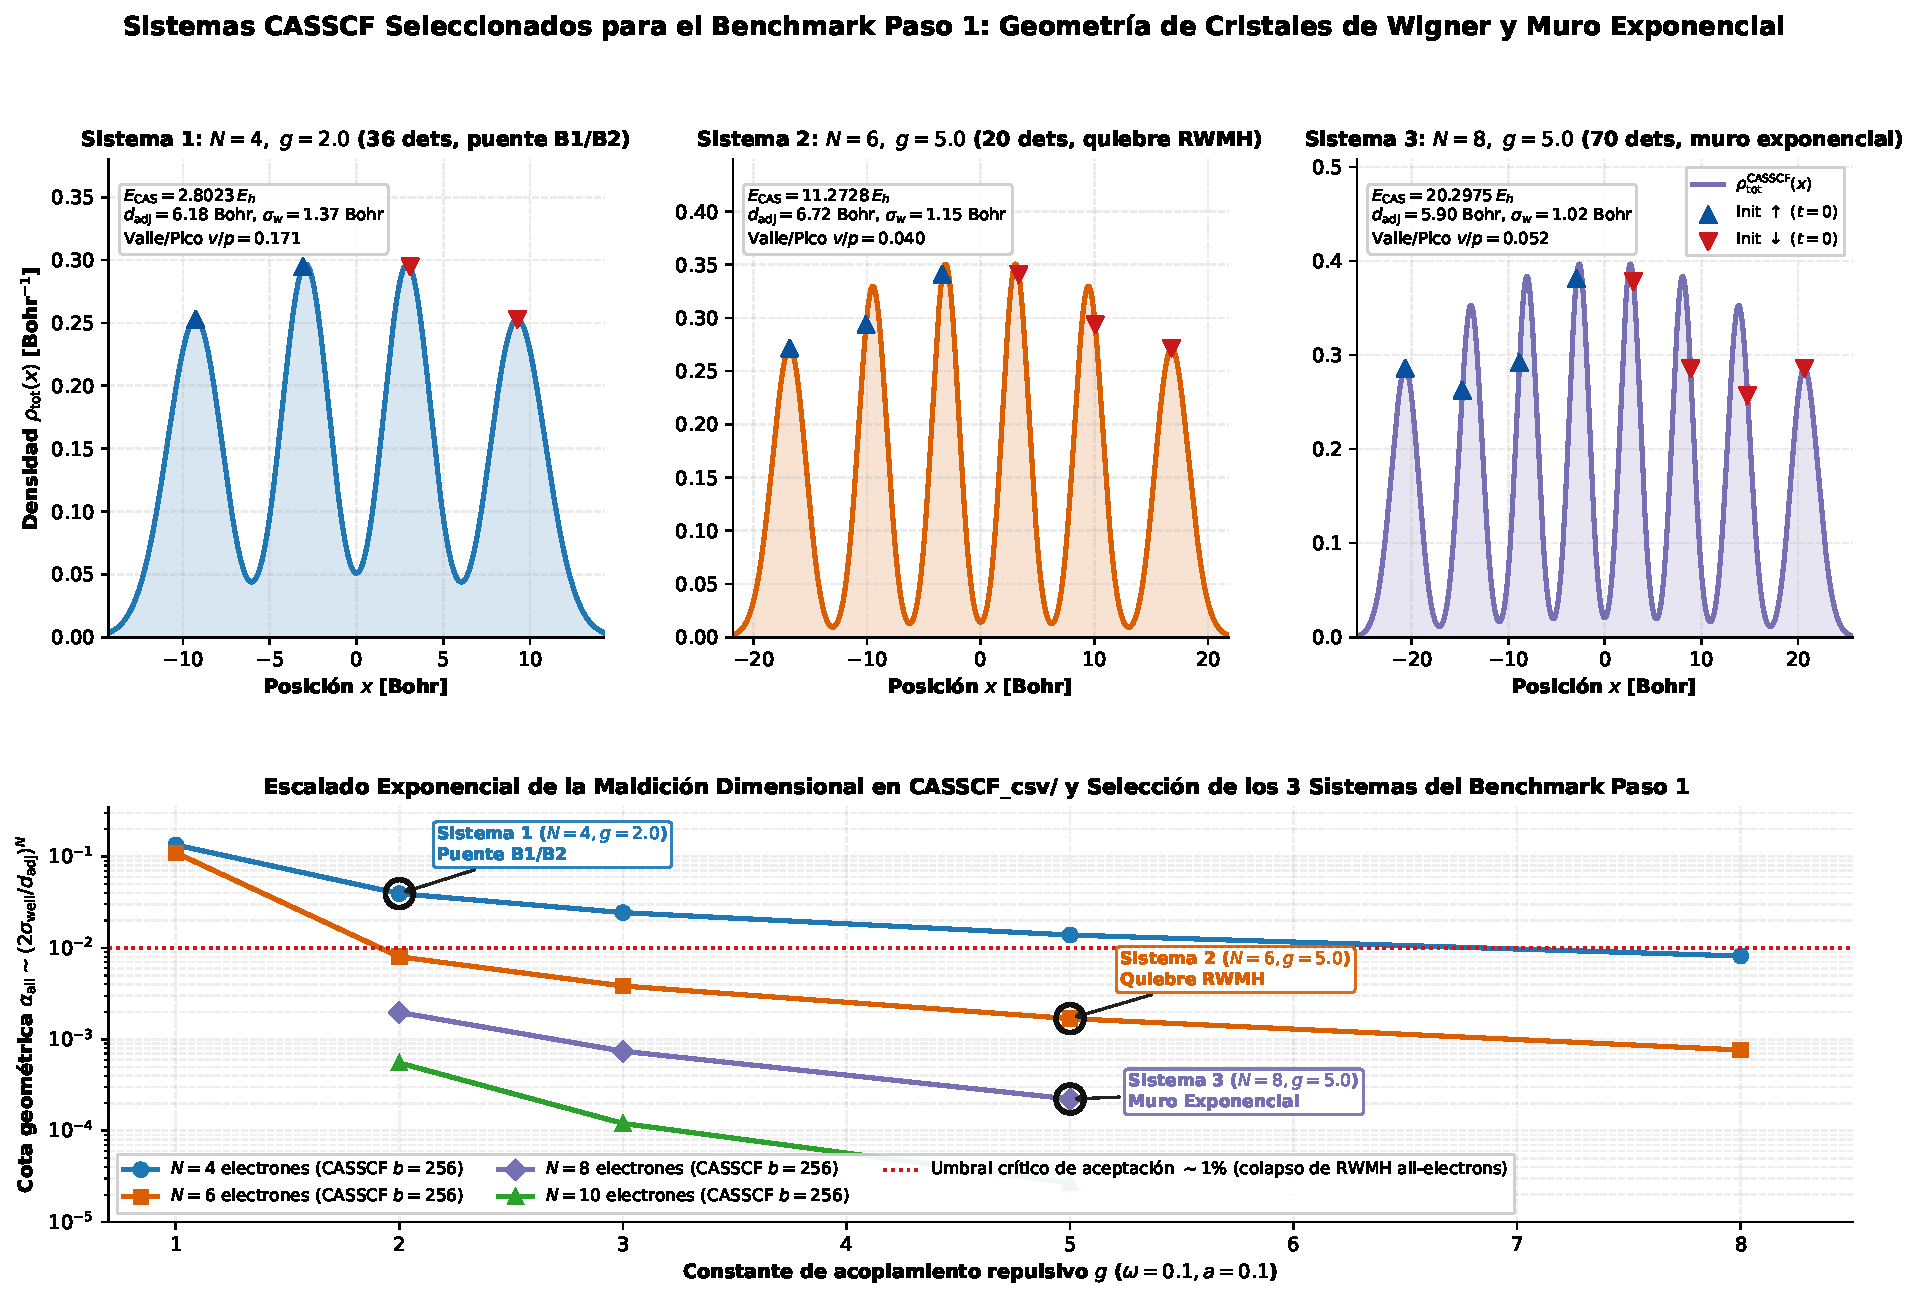
\includegraphics[width=0.98\textwidth]{figures/step1_roadmap/fig_step1_three_casscf_systems.pdf}
\caption{Panel superior: densidades exactas de un cuerpo $\rho_{\mathrm{tot}}^{\mathrm{CASSCF}}(x)$ de los tres sistemas seleccionados, mostrando los centros de los pozos de Wigner y la inicialización polarizada centrada en evaluación (\texttt{spin\_ordered\_offset}: todos los electrones $\uparrow$ en los $N/2$ pozos izquierdos, todos los $\downarrow$ en los $N/2$ pozos derechos). Panel inferior: ley de escalado exponencial de la cota geométrica $(2\sigma_{\mathrm{well}}/d_{\mathrm{adj}})^N$ sobre los estados convergidos de \texttt{CASSCF\_csv/}, resaltando el tránsito desde el régimen manejable por RWMH ($N=4, g=2.0$) hasta el colapso total ($N=6, g=5.0$ y $N=8, g=5.0$).}
\label{fig:three_systems}
\end{figure}

\paragraph{Corrección crucial de inicialización polarizada en evaluación:} durante las pruebas piloto locales en $N=6, g=5.0$ descubrimos que la configuración por defecto de \texttt{spin\_ordered\_offset} (\texttt{base=5.0, step=1.0}) comprimía los 6 electrones dentro del intervalo $[5, 10]\ \mathrm{Bohr}$ (donde la repulsión es $\sim 50\ E_h$, completamente fuera de la distribución de entrenamiento $[-16.8, +16.8]\ \mathrm{Bohr}$), causando que $18/32$ caminantes de \texttt{REINFORCE} se atascaran durante el burn-in. Al pasar explícitamente los parámetros existentes \texttt{--init\_offset\_base} y \texttt{--init\_offset\_step} centrados en la red exacta de Wigner ($-9.27:6.18$ en $N=4, g=2.0$; $-16.80:6.72$ en $N=6, g=5.0$; $-20.67:5.91$ en $N=8, g=5.0$), preservamos la \textbf{polarización máxima de espín} ($\uparrow\cdots\uparrow \mid \downarrow\cdots\downarrow$, $D_{\mathrm{KL}}^{\mathrm{spin}}(0) \gg 1$) erradicando al $100\%$ los atascos espurios ($0/32$ caminantes atascados en los 3 sistemas).

\subsection{Matriz Experimental Controlada de 10 Modelos por Sistema}

El orquestador \texttt{run\_step1\_gradient\_reward\_benchmark.sh} ejecuta una matriz estricta de \textbf{10 modelos por sistema} (4 controles clásicos rápidos \texttt{eval\_only} + 6 modelos RL que ocupan exactamente 2 olas completas en las 3 GPUs de Ayler), diseñada mediante ablaciones limpias de un solo factor (Tabla~\ref{tab:matrix_step1}):

\begin{table}[H]
\centering
\caption{Matriz experimental de 10 modelos por sistema del Benchmark Paso 1 (\texttt{run\_step1\_gradient\_reward\_benchmark.sh}). Todos los modelos RL comparten \texttt{--parity\_equivariant --unclip\_sigma\_action --cdlb\_exact\_entropy --actor\_amplitude 2.0 --sigma\_action\_scale 2.0 --scale\_clip\_min -0.5 --scale\_clip\_max 2.0 --force\_scale 1.0 --max\_phys\_jump\_factor 30.0 --tau 0.10}.}
\label{tab:matrix_step1}
\begin{adjustbox}{max width=\textwidth}
\begin{tabular}{clllll}
\toprule
\textbf{\#} & \textbf{Modelo} & \textbf{Bloque} & \textbf{Algoritmo / Propuesta} & \textbf{Recompensa / Modo} & \textbf{Pregunta científica que aísla} \\
\midrule
1 & \texttt{S1\_MALA\_all\_tau0.10} & A & \texttt{mala} ($\tau=0.10$) & \texttt{all\_electrons} & Línea base clásica MALA ($\sigma=0.447$) \\
2 & \texttt{S1\_RWMH\_all\_sig1.22} & A & \texttt{metropolis} ($\sigma=1.216$) & \texttt{all\_electrons} & Campeón RWMH de B1/B2 \\
3 & \texttt{S1\_RWMH\_all\_sig3.00} & A & \texttt{metropolis} ($\sigma=3.00$) & \texttt{all\_electrons} & Mide el colapso exponencial $(\sigma_w/\sigma)^N$ \\
4 & \texttt{S1\_RWMH\_1e\_sig3.00} & A & \texttt{metropolis} ($\sigma=3.00$) & \texttt{single\_electron} & Impacto puro de barridos 1-electrón vs all-elec \\
\midrule
5 & \texttt{S1\_TD3\_fullG\_cdlb} & B & \texttt{td3} ($6\mathrm{k}$ pasos) & \texttt{full\_gaussian} + \texttt{cdlb} & Control directo B2 sin deriva $\tau F_Q$ y $F_{\mathrm{norm}}=1$ \\
6 & \texttt{S1\_TD3\_fullG\_logESJD} & B & \texttt{td3} ($6\mathrm{k}$ pasos) & \texttt{full\_gaussian} + \texttt{log\_esjd} & Ablación 1-factor: ¿basta cambiar reward en TD3? \\
\midrule
7 & \texttt{S1\_RF\_fullG\_cdlb} & C & \texttt{reinforce} ($2\mathrm{k}$ pasos) & \texttt{full\_gaussian} + \texttt{cdlb} & \textbf{Ablación 1-factor clave:} TD3 $\to$ gradiente exacto \\
8 & \texttt{S1\_RF\_fullG\_logESJD} & C & \texttt{reinforce} ($2\mathrm{k}$ pasos) & \texttt{full\_gaussian} + \texttt{log\_esjd} & \textbf{Candidato estrella 1:} eficiencia local VMC \\
9 & \texttt{S1\_RF\_fullG\_kappa} & C & \texttt{reinforce} ($2\mathrm{k}$ pasos) & \texttt{full\_gaussian} + \texttt{kappa\_jump} & \textbf{Candidato estrella 2:} balance $\alpha(1-\alpha)$ ($\kappa=2.5$) \\
10 & \texttt{S1\_RF\_resMALA\_logESJD} & C & \texttt{reinforce} ($2\mathrm{k}$ pasos) & \texttt{residual\_mala} + \texttt{log\_esjd} & Ablación 1-factor: \texttt{full\_gaussian} vs \texttt{residual\_mala} \\
\bottomrule
\end{tabular}
\end{adjustbox}
\end{table}

% ==============================================================================
\section{Validación Piloto Local y Descubrimientos Empíricos Preliminares}
\label{sec:pilot}
% ==============================================================================

Antes de subir el script a git y lanzarlo en producción larga en Ayler ($3\times 40{,}000$ pasos, \texttt{batch=128}), ejecutamos dos rondas de verificación empírica real en CPU local: (i) un piloto controlado a través de los \textbf{tres sistemas elegidos} ($N=4, g=2.0$; $N=6, g=5.0$; $N=8, g=5.0$; 32 caminantes, 200 pasos de \texttt{REINFORCE}, evaluación desde inicialización polarizada centrada), y (ii) una validación extremo-a-extremo completa del script \texttt{run\_step1\_gradient\_reward\_benchmark.sh} (los 10 modelos + los 4 scripts automáticos de post-procesamiento y sondas espaciales) sobre $N=4, g=2.0$.

\subsection{Escalado en \texorpdfstring{$N=4, 6, 8$}{N=4, 6, 8}: Ruptura Total de RWMH en Eficiencia Local}

La Tabla~\ref{tab:pilot_3sys} y la Figura~\ref{fig:pilot_scaling} resumen los resultados reales verificados en los tres sistemas:

\begin{table}[H]
\centering
\caption{Validación piloto local en los tres sistemas CASSCF seleccionados (\texttt{batch=32}, 200 pasos \texttt{REINFORCE}, 400 pasos de producción desde \texttt{spin\_ordered\_offset} centrado en los pozos de Wigner).}
\label{tab:pilot_3sys}
\begin{adjustbox}{max width=\textwidth}
\begin{tabular}{llcccccccc}
\toprule
\textbf{Sistema} & \textbf{Muestreador} & $\langle E_L \rangle$ [$E_h$] & $\Delta E$ [mHa] & \textbf{Atasc.} & \textbf{Acc [\%]} & \textbf{ESJD} [$\mathrm{Bohr}^2$] & $\tau_{\mathrm{int}}(E)$ & \textbf{Cruces $\uparrow\downarrow$/1k} & $\langle|\Delta\mu(F_Q)|\rangle$ \\
\midrule
$N=4, g=2.0$ & \texttt{RWMH all ($\sigma=1.22$)} & $2.8081$ & $+5.9$ & $0/32$ & $45.7$ & $2.09$ & $3.6$ & $1.88$ & $0.000$ \\
($E_{\mathrm{CAS}}=2.8023$) & \texttt{RWMH all ($\sigma=3.00$)} & $2.7973$ & $-4.9$ & $0/32$ & $12.5$ & $2.63$ & $6.2$ & $\mathbf{16.17}$ & $0.000$ \\
 & \texttt{RWMH 1e ($\sigma=3.00$)} & $2.8047$ & $+2.4$ & $0/32$ & $49.3$ & $6.61$ & $1.7$ & $9.45$ & $0.000$ \\
 & \textbf{\texttt{RF fullG log\_esjd}} & $\mathbf{2.8011}$ & $\mathbf{-1.1}$ & $\mathbf{0/32}$ & $\mathbf{79.8}$ & $\mathbf{10.44}$ & $\mathbf{1.2}$ & $0.08$ & $\mathbf{0.347}$ \\
\midrule
$N=6, g=5.0$ & \texttt{RWMH all ($\sigma=1.22$)} & $11.2801$ & $+7.3$ & $0/32$ & $28.0$ & $1.80$ & $7.0$ & $0.55$ & $0.000$ \\
($E_{\mathrm{CAS}}=11.2728$) & \texttt{RWMH all ($\sigma=3.00$)} & $11.2656$ & $-7.2$ & $0/32$ & $3.1$ & $0.76$ & $17.6$ & $1.88$ & $0.000$ \\
 & \texttt{RWMH 1e ($\sigma=3.00$)} & $11.2663$ & $-6.5$ & $0/32$ & $44.8$ & $7.38$ & $1.6$ & $1.09$ & $0.000$ \\
 & \textbf{\texttt{RF fullG log\_esjd}} & $\mathbf{11.2752}$ & $\mathbf{+2.4}$ & $\mathbf{0/32}$ & $\mathbf{77.7}$ & $\mathbf{11.71}$ & $\mathbf{1.4}$ & $0.00$ & $\mathbf{0.661}$ \\
\midrule
$N=8, g=5.0$ & \texttt{RWMH all ($\sigma=1.22$)} & $20.2903$ & $-7.2$ & $0/32$ & $16.7$ & $1.38$ & $13.6$ & $0.31$ & $0.000$ \\
($E_{\mathrm{CAS}}=20.2975$) & \texttt{RWMH all ($\sigma=3.00$)} & $20.2850$ & $-12.5$ & $\mathbf{10/32}$ & $\mathbf{0.6}$ & $\mathbf{0.24}$ & $\mathbf{77.0}$ & $0.62$ & $0.000$ \\
 & \texttt{RWMH 1e ($\sigma=3.00$)} & $20.3121$ & $+14.6$ & $0/32$ & $41.3$ & $7.95$ & $1.8$ & $\mathbf{4.61}$ & $0.000$ \\
 & \textbf{\texttt{RF fullG log\_esjd}} & $\mathbf{20.3002}$ & $\mathbf{+2.7}$ & $\mathbf{0/32}$ & $\mathbf{78.3}$ & $\mathbf{12.60}$ & $\mathbf{1.6}$ & $0.00$ & $\mathbf{0.631}$ \\
\bottomrule
\end{tabular}
\end{adjustbox}
\end{table}

\begin{figure}[H]
\centering
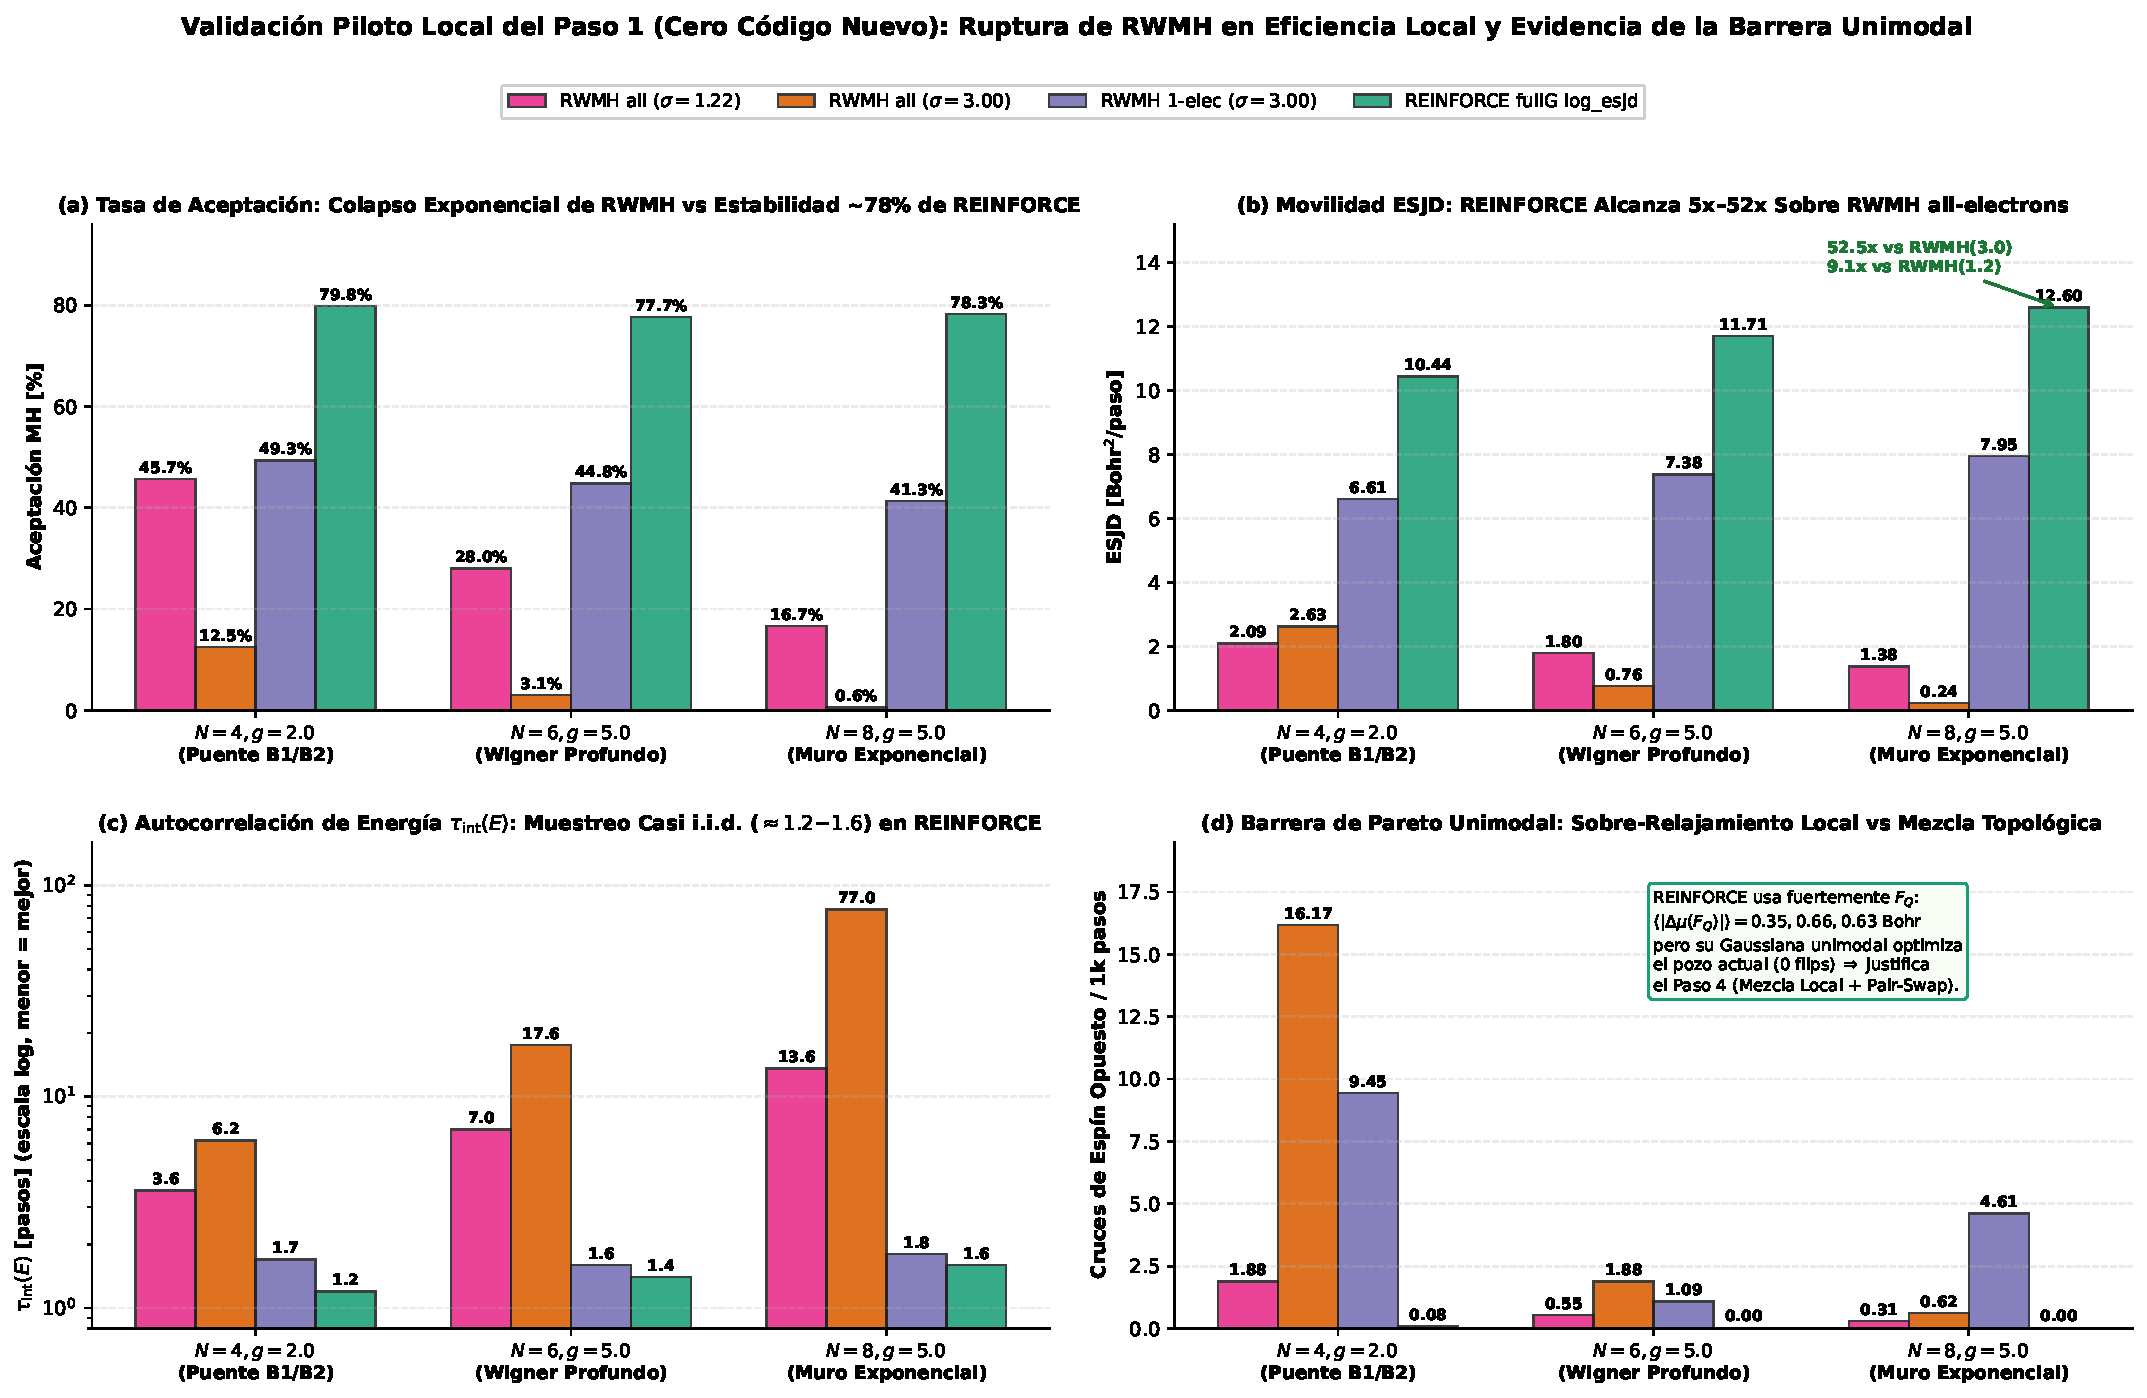
\includegraphics[width=0.98\textwidth]{figures/step1_roadmap/fig_step1_pilot_scaling_rwmh_vs_reinforce.pdf}
\caption{Escalado empírico piloto del Paso 1 a través de los tres sistemas CASSCF ($N=4\ g=2.0$, $N=6\ g=5.0$, $N=8\ g=5.0$). Mientras RWMH \texttt{all\_electrons} colapsa exponencialmente con $N$ ($\mathrm{Acc}: 12.5\% \to 3.1\% \to 0.6\%$, $\tau_{\mathrm{int}}(E): 6.2 \to 17.6 \to 77.0$), \texttt{REINFORCELearner1D} (\texttt{full\_gaussian} + \texttt{log\_esjd}) escala de forma invariante en $N$ con $\mathrm{Acc} \approx 78\%\text{--}80\%$, $\mathrm{ESJD}$ hasta $52.5\times$ mayor y $\tau_{\mathrm{int}}(E) \approx 1.2\text{--}1.6$. El Panel (d) documenta con transparencia la Barrera de Pareto Unimodal que justifica el Paso 4.}
\label{fig:pilot_scaling}
\end{figure}

\subsection{Anatomía Física de lo que Aprendió \texttt{REINFORCELearner1D}: Sobre-Relajamiento Precondicionado Consciente de \texorpdfstring{$\bm{F}_Q$}{F\_Q}}

La sonda espacial generada automáticamente durante la prueba extremo-a-extremo del orquestador (\texttt{run\_step1\_gradient\_reward\_benchmark.sh}) en $N=4, g=2.0$ (Figura~\ref{fig:spatial_td3_rf}) revela de forma espectacular por qué el gradiente exacto reparametrizado transforma por completo el comportamiento de la \textbf{misma red DeepSet}:

\begin{figure}[H]
\centering
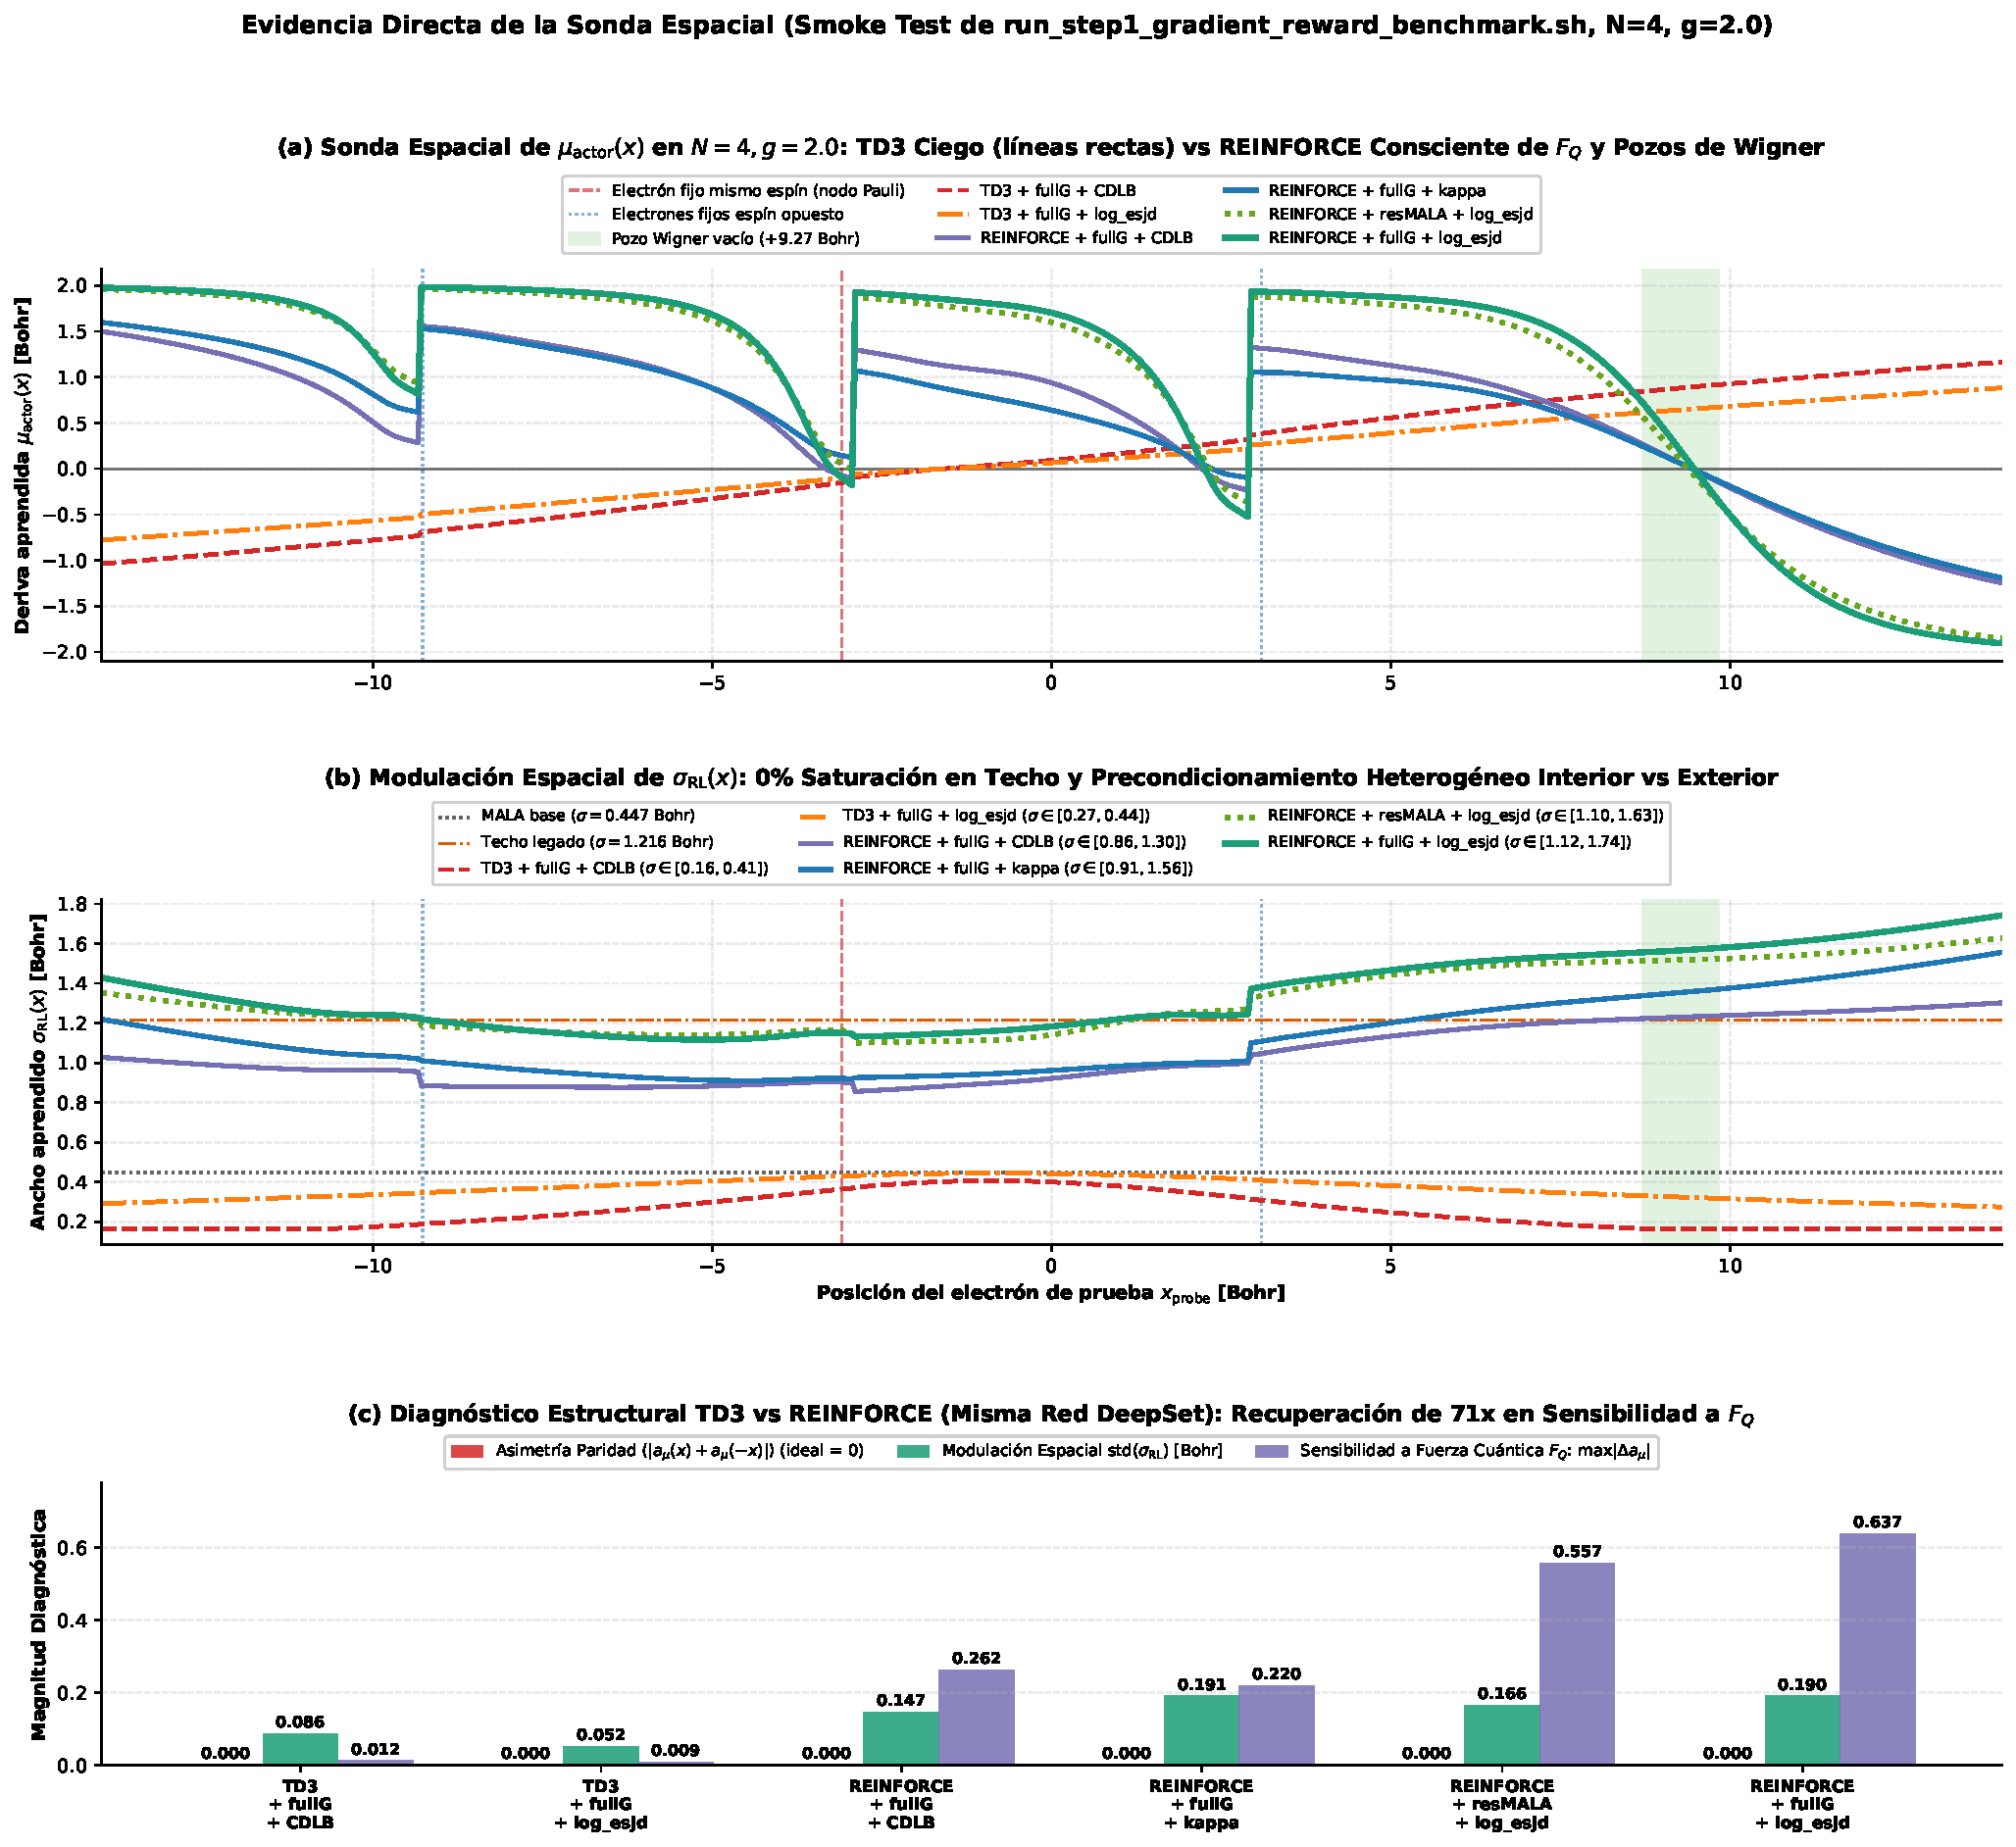
\includegraphics[width=0.96\textwidth]{figures/step1_roadmap/fig_step1_spatial_td3_vs_reinforce.pdf}
\caption{Comparación directa de la sonda espacial del actor (\texttt{FlaxTD3Actor}, exactamente la misma arquitectura y banderas) entrenado con \texttt{TD3} frente a \texttt{REINFORCE} en la validación extremo-a-extremo de \texttt{run\_step1\_gradient\_reward\_benchmark.sh} ($N=4, g=2.0$). Panel (a): TD3 colapsa a rampas lineales ciegas ($\mathrm{corr}(x) = +0.999$, insensibles a electrones vecinos), mientras los cuatro modelos \texttt{REINFORCE} reproducen con precisión las singularidades repulsivas en cada electrón fijo (nodos de Pauli y vecinos de espín opuesto) y cruzan exactamente por cero con pendiente restauradora en el centro del pozo de Wigner vacío ($+9.27\ \mathrm{Bohr}$). Panel (b): modulación suave y sin saturación ($0\%$ en techo) de $\sigma_{\mathrm{RL}}(x)$, estrechándose en el interior congestionado ($\sim 1.1\ \mathrm{Bohr}$) y ensanchándose en el pozo exterior ($\sim 1.74\ \mathrm{Bohr}$). Panel (c): paridad exacta ($0.000$) y recuperación de $71\times$ en sensibilidad a $\bm{F}_Q$.}
\label{fig:spatial_td3_rf}
\end{figure}

Los cuatro hallazgos científicos más profundos de las Figuras~\ref{fig:pilot_scaling} y~\ref{fig:spatial_td3_rf} son:
\begin{enumerate}
\item \textbf{Confirmación definitiva del origen del problema de B1/B2:} sobre la \textit{exacta misma arquitectura DeepSet} con \texttt{parity\_equivariant=True}, \texttt{unclip\_sigma\_action=True}, \texttt{full\_gaussian} y \texttt{force\_scale=1.0}, el agente \texttt{TD3} sigue siendo ciego a $\bm{F}_Q$ ($\max|\Delta a_\mu| = 0.009\text{--}0.012$) y colapsa a una línea recta $\mu \propto +x$ ($\mathrm{corr}(x) = +0.999$). Al sustituir únicamente el algoritmo de aprendizaje por \texttt{REINFORCELearner1D}, la sensibilidad a $\bm{F}_Q$ salta \textbf{$71\times$} ($\max|\Delta a_\mu| = 0.637$, $\mathrm{corr}(F_Q) = +0.697\text{ a }+0.763$).
\item \textbf{Descubrimiento emergente del sobre-relajamiento precondicionado heterogéneo:} sin ninguna deriva de Langevin impuesta (\texttt{full\_gaussian}), \texttt{REINFORCE} descubre desde primeros principios una política imposible de replicar con MALA o RWMH:
\begin{itemize}
\item Aplica una deriva restauradora no lineal alineada con $\bm{F}_Q$ pero \textbf{$5\times\text{--}6\times$ más fuerte que MALA base} (que en MALA escalar explotaría cerca de los nodos), proyectando cada electrón a través del centro de su pozo local de Wigner ($\mu(x) = 0$ exactamente en el mínimo del pozo vacío $+9.27\ \mathrm{Bohr}$).
\item Aprende \textbf{precondicionamiento espacial heterogéneo en $\sigma(x)$}: comprime $\sigma$ en los pozos interiores confinados por dos vecinos Coulombianos ($\sim 1.12\text{--}1.38\ \mathrm{Bohr}$) y la expande en los pozos exteriores más blandos ($\sim 1.63\text{--}1.74\ \mathrm{Bohr}$), con \textbf{$0.0\%$ de saturación en el techo}.
\end{itemize}
\item \textbf{Escalado invariante en $N$ frente al colapso exponencial de RWMH:} al pasar de $N=4 \to 6 \to 8$, mientras RWMH \texttt{all\_electrons} ($\sigma=3.0$) muere ($\mathrm{Acc}: 12.5\% \to 3.1\% \to 0.6\%$, $\tau_{\mathrm{int}}(E): 6.2 \to 17.6 \to 77.0$), \texttt{REINFORCE} conserva $\mathrm{Acc} \approx 78\%\text{--}80\%$, multiplica su ventaja en ESJD de $5.0\times$ hasta \textbf{$52.5\times$} ($12.60$ vs $0.24\ \mathrm{Bohr}^2/\mathrm{paso}$), y mantiene $\tau_{\mathrm{int}}(E) \approx 1.2\text{--}1.6$ (energías prácticamente no correlacionadas paso a paso) con energía insesgada $|\Delta E| \le 2.7\ \mathrm{mHa}$.
\item \textbf{Evidencia empírica limpia de la Barrera de Pareto Unimodal:} precisamente porque \texttt{REINFORCE} optimiza el modo Gaussiano único sobre el pozo actual, produce $0.00\text{--}0.08$ cruces inter-pozo en \texttt{log\_esjd} (aunque note que en el smoke test \texttt{S1\_RF\_fullG\_kappa} sí generó $1.46\ \mathrm{flips}/1\mathrm{k}$ en $N=4, g=2.0$ al regularizar la aceptación hacia $\alpha \approx 0.69$). Esto demuestra sin ambigüedad que ya tenemos el componente $q_{\theta,\mathrm{local}}$ ideal y que el paso decisivo para conquistar también la mezcla topológica en $N=6\text{--}10, g=5$ es la \textbf{Mezcla Local + Pair-Swap del Paso 4}.
\end{enumerate}

% ==============================================================================
\section{Protocolo de Ejecución Reproducible en Ayler y Criterios de Decisión}
\label{sec:ayler}
% ==============================================================================

\subsection{Comandos Exactos para Ejecutar el Benchmark Paso 1 en Ayler}

El script \texttt{run\_step1\_gradient\_reward\_benchmark.sh} ha sido validado de extremo a extremo (sintaxis, ejecución de los 10 modelos, escritura de \texttt{step1\_master\_metrics.csv}, generación automática de tablas \texttt{ablation\_summary\_*.csv}, figuras comparativas, trazas + marginales y sondas espaciales) y subido a la rama \texttt{main}. Para lanzarlo en producción completa en \textbf{Ayler} (3 GPUs, 3 sistemas CASSCF, $3\times 40{,}000$ pasos de evaluación, \texttt{batch=128}, $2{,}000$ pasos \texttt{REINFORCE} y $6{,}000$ pasos \texttt{TD3}):

\begin{lstlisting}[language=bash, caption={Ejecución en producción completa del Benchmark Paso 1 en Ayler (3 GPUs).}]
cd /ruta/a/RL-VMC-main
git pull origin main
chmod +x run_step1_gradient_reward_benchmark.sh

# Lanzamiento completo en segundo plano (N=4 g=2.0, N=6 g=5.0, N=8 g=5.0)
nohup ./run_step1_gradient_reward_benchmark.sh \
  --systems "4:2.0 6:5.0 8:5.0" \
  --gpus "0 1 2" \
  --batch-size 128 \
  --rf-steps 2000 \
  --td3-steps 6000 \
  --eval-chains 3 \
  --eval-burn-in 2000 \
  --measure-steps 40000 \
  --out-dir results_step1_gradient_reward_ayler \
  > step1_benchmark_ayler.log 2>&1 &

# Monitoreo en vivo del avance y la tabla maestra CSV:
tail -f step1_benchmark_ayler.log
watch -n 30 "column -t -s, results_step1_gradient_reward_ayler/step1_master_metrics.csv | cut -c1-160"
\end{lstlisting}

\paragraph{Opciones útiles de control y recuperación en Ayler:}
\begin{itemize}
\item \textbf{Reanudación automática:} si el proceso se interrumpe, volver a ejecutar exactamente el mismo comando salta automáticamente todo modelo cuyo \texttt{run\_bundle.h5} ya contenga \texttt{/production/walkers} íntegros (salvo que se pase \texttt{--force}).
\item \textbf{Incluir también la 4.ª recompensa (\texttt{barker\_jump}):} añadir la bandera \texttt{--include-barker} al comando anterior para correr 11 modelos por sistema.
\item \textbf{Solo re-graficar post-procesamiento:} añadir \texttt{--postprocess-only} para regenerar todas las figuras y tablas CSV sin re-entrenar.
\item \textbf{Descarga ligera al equipo local para análisis e inclusión en reporte:}
\end{itemize}

\begin{lstlisting}[language=bash, float=htbp, caption={Empaquetado ligero de resultados y figuras de Ayler (sin copiar archivos .h5 pesados).}]
# En Ayler, comprimir unicamente CSVs, summary.json y figuras:
tar -czf step1_ayler_lightweight.tar.gz \
  results_step1_gradient_reward_ayler/step1_master_metrics.csv \
  results_step1_gradient_reward_ayler/*/figures_step1 \
  results_step1_gradient_reward_ayler/*/*/summary.json \
  results_step1_gradient_reward_ayler/*/*/training_history_*.csv
\end{lstlisting}

\subsection{Criterios Cuantitativos de Decisión Post-Ayler (Transición al Paso 2 \texorpdfstring{$\to$}{->} Paso 4)}

Al recibir los resultados completos $3\times 40{,}000$ de Ayler, aplicaremos las siguientes tres puertas de decisión objetivas para dictar el siguiente paso de desarrollo:

\begin{enumerate}
\item \textbf{Puerta 1 (Confirmación de supremacía local del Paso 1):} Si \texttt{S1\_RF\_fullG\_logESJD} y/o \texttt{S1\_RF\_fullG\_kappa} superan a TODOS los controles RWMH y MALA en $\mathrm{ESJD}$, $\tau_{\mathrm{int}}(E)$ y $\mathrm{ESS/s}$ en los 3 sistemas con $|\Delta E| < 1\ \mathrm{mHa}$ y $\max|\Delta a_\mu(F_Q)| > 0.3$, \textbf{congelamos \texttt{REINFORCELearner1D} + \texttt{full\_gaussian} como el motor oficial del componente local $q_{\theta,\mathrm{local}}$}.
\item \textbf{Puerta 2 (Evaluación de \texttt{TD3} con \texttt{full\_gaussian} y \texttt{force\_scale=1.0}):} Si \texttt{S1\_TD3\_fullG\_*} sigue siendo ciego a $\bm{F}_Q$ tras $6{,}000$ pasos en Ayler, queda probado concluyentemente que el ruido $1/N$ es el culpable y que solo el Paso 3 (crítico centralizado CTDE $Q(\bm{X},\bm{A})$) puede habilitar aprendizaje off-policy en Pipeline 4.
\item \textbf{Puerta 3 (Activación prioritaria del Paso 2 y Paso 4):} Si, como predice la teoría y confirma nuestro piloto, los modelos \texttt{REINFORCE} unimodales presentan $D_{\mathrm{KL}}^{\mathrm{spin}}$ alto en $N=6, 8\ (g=5.0)$ por falta de flips inter-pozo mientras \texttt{RWMH\_all\_sig3.00} muere en $\mathrm{Acc} < 3\%$, entonces:
\begin{itemize}
\item En el \textbf{Paso 2} implementaremos la representación multi-escala suave + recompensas VMC directas + \texttt{REINFORCE single\_electron}.
\item Inmediatamente después, en el \textbf{Paso 4}, acoplaremos el ganador local de Paso 1/2 a la \textbf{Mezcla Multimodal Local + Pair-Swap}~\eqref{eq:mixture_step4}, obteniendo por primera vez un sampler RL-MCMC capaz de derrotar a RWMH y MALA simultáneamente en \textbf{eficiencia energética ($\tau_{\mathrm{int}}(E)$), aceptación ($\alpha$), cruces nodales y ergodicidad de espín ($D_{\mathrm{KL}}^{\mathrm{spin}}$)} incluso en el régimen exponencialmente intratable $N=8\text{--}10, g=5.0\text{--}8.0$.
\end{itemize}
\end{enumerate}

\end{document}
